
\section{Benchmark Composition}
\label{app:architectures}

Table~\ref{tab:arch_detail} reports the per-architecture composition of \fastkernels{}: the reference HuggingFace checkpoint, default inference dtype, and the number of L1 (primitive), L2 (fused/composite), L3 (layer/block) and L4 (end-to-end) tasks each architecture uses.

\paragraph{Counting rule.}
A task is one module file under \texttt{tasks/baseline/L$n$/} that defines at least one benchmarkable \texttt{nn.Module} and is reachable, through the import graph, from at least one of the 47 L4 architectures; it is counted once even when it ships a CUDA sidecar (17 tasks do) or defines several module classes.
Twelve function-only helper kernels (e.g., Triton attention-merge and causal-convolution kernels) are called from inside other tasks and are optimized through them, so they are not counted separately.
This yields 108 L1, 155 L2, and 74 L3 tasks plus 47 L4 models, 384 in total.
L4 counts one task per end-to-end architecture: the encoder sub-models that some pipelines import (the CLIP and T5 text encoders, the Qwen2.5-VL vision encoder) are part of those pipelines' L4 tasks, and the L1--L3 set is identical with or without DeepSeek-V3.2, whose modules GLM-5.2 builds on.
Because tasks are shared, the per-architecture columns of Table~\ref{tab:arch_detail} sum to more than these totals.

\begin{table}[H]
  \centering
  \caption{Full architecture composition of \fastkernels{}. L1--L4 report the number of primitive, fused/composite, layer/block-level, and end-to-end tasks each architecture uses, under the counting rule above (L4 is always 1 by construction). \emph{Reference} is the HuggingFace checkpoint or upstream repository the L4 pipeline tracks; \emph{dtype} is the default inference dtype.}
  \label{tab:arch_detail}
  \scriptsize
  \setlength{\tabcolsep}{3pt}
  \begin{tabular}{@{}ll>{\raggedright\arraybackslash}p{4.5cm}lcccc@{}}
  \toprule
  \textbf{Category} & \textbf{Architecture} & \textbf{Reference} & \textbf{dtype} & \textbf{L1} & \textbf{L2} & \textbf{L3} & \textbf{L4} \\
  \midrule
  \multirow{7}{*}{Dense \& MoE LLMs}
   & Llama-3.1          & \texttt{meta-llama/\allowbreak Llama-3.1-8B-Instruct}    & BF16 & 13 & 6 & 1 & 1 \\
   & GLM-5.2            & \texttt{nvidia/\allowbreak GLM-5.2-NVFP4}                & NVFP4 & 31 & 11 & 1 & 1 \\
   & Mixtral            & \texttt{mistralai/\allowbreak Mixtral-8x7B-Instruct-v0.1} & BF16 & 19 & 8 & 1 & 1 \\
   & BitNet 1.58b       & \texttt{microsoft/\allowbreak bitnet-b1.58-2B-4T}        & W1.58/BF16 & 13 & 5 & 1 & 1 \\
   & GPT-OSS (MXFP4)    & \texttt{openai/\allowbreak gpt-oss-120b}                 & MXFP4 & 13 & 8 & 1 & 1 \\
   & EAGLE-3            & \texttt{jamesliu1/\allowbreak sglang-EAGLE3-Llama-3.1-Instruct-8B} & BF16 & 13 & 4 & 0 & 1 \\
   & Gemma-4            & \texttt{google/\allowbreak gemma-4-26B-A4B-it}           & BF16 & 20 & 8 & 1 & 1 \\
  \midrule
  \multirow{9}{*}{\makecell[l]{Linear Attention\\\& New Archs}}
   & Mamba              & \texttt{state-spaces/\allowbreak mamba-2.8b-hf}          & BF16 & 7  & 3 & 1 & 1 \\
   & Mamba2             & \texttt{mistralai/\allowbreak Mamba-Codestral-7B-v0.1}   & BF16 & 9  & 3 & 1 & 1 \\
   & RWKV-7             & \texttt{fla-hub/\allowbreak rwkv7-2.9B-g1}               & BF16 & 11 & 2 & 1 & 1 \\
   & GLA                & \texttt{fla-hub/\allowbreak gla-2.7B-100B}               & BF16 & 11 & 2 & 1 & 1 \\
   & RetNet             & \texttt{fla-hub/\allowbreak retnet-2.7B-100B}            & BF16 & 11 & 2 & 1 & 1 \\
   & Qwen-3-Next        & \texttt{Qwen/\allowbreak Qwen3-Next-80B-A3B-Instruct}    & BF16 & 22 & 7 & 1 & 1 \\
   & Kimi-Linear        & \texttt{moonshotai/\allowbreak Kimi-Linear-48B-A3B-Instruct} & BF16 & 25 & 9 & 1 & 1 \\
   & TTT-E2E            & \texttt{test-time-training/e2e}                          & BF16 & 8  & 3 & 1 & 1 \\
   & Jamba              & \texttt{ai21labs/\allowbreak AI21-Jamba-Mini-1.7}        & BF16 & 20 & 8 & 1 & 1 \\
  \midrule
  \multirow{6}{*}{\makecell[l]{Vision / Video /\\Audio}}
   & FLUX.1-Dev         & \texttt{black-forest-labs/\allowbreak FLUX.1-dev}        & BF16 & 16 & 10 & 3 & 1 \\
   & HunyuanVideo-1.5   & \texttt{hunyuanvideo-community/\allowbreak HunyuanVideo-1.5} & BF16 & 24 & 15 & 4 & 1 \\
   & SDXL               & \texttt{stabilityai/\allowbreak stable-diffusion-xl-base-1.0} & FP16 & 8  & 8  & 3 & 1 \\
   & SAM3.1             & \texttt{facebook/\allowbreak sam3.1}                     & BF16 & 8  & 6  & 8 & 1 \\
   & Whisper            & \texttt{openai/\allowbreak whisper-large-v3}             & FP16 & 13 & 6  & 2 & 1 \\
   & CosyVoice3         & \texttt{FunAudioLLM/\allowbreak Fun-CosyVoice3-0.5B-2512} & BF16 & 14 & 9  & 2 & 1 \\
  \midrule
  \multirow{7}{*}{\makecell[l]{Multimodal \&\\Encoders}}
   & Qwen2-VL           & \texttt{Qwen/\allowbreak Qwen2-VL-7B-Instruct}           & BF16 & 20 & 10 & 2 & 1 \\
   & Qwen3-VL-8B        & \texttt{Qwen/\allowbreak Qwen3-VL-8B-Instruct}           & BF16 & 27 & 13 & 3 & 1 \\
   & Qwen3-VL-235B      & \texttt{Qwen/\allowbreak Qwen3-VL-235B-A22B-Instruct-FP8} & FP8  & 27 & 13 & 3 & 1 \\
   & Qwen-2.5-Omni      & \texttt{Qwen/\allowbreak Qwen2.5-Omni-7B}                & BF16 & 20 & 10 & 2 & 1 \\
   & SigLIP-2           & \texttt{google/\allowbreak siglip2-so400m-patch16-naflex} & BF16 & 3  & 3  & 1 & 1 \\
   & DINOv3             & \texttt{facebook/\allowbreak dinov3-vit7b16-pretrain-lvd1689m} & BF16 & 4  & 2  & 1 & 1 \\
   & SwinV2             & \texttt{timm/\allowbreak swinv2\_large\_window12\_192.ms\_in22k} & FP32 & 4 & 3 & 2 & 1 \\
  \midrule
  \multirow{5}{*}{\makecell[l]{Edge \&\\Detection}}
   & MobileNetV4        & \texttt{timm/\allowbreak mobilenetv4\_conv\_medium.\allowbreak e500\_r256\_in1k} & FP32 & 5  & 2  & 1 & 1 \\
   & ConvNeXtV2         & \texttt{facebook/\allowbreak convnextv2-base-22k-384}    & FP32 & 7  & 1  & 1 & 1 \\
   & EfficientNetV2     & \texttt{timm/\allowbreak efficientnetv2\_rw\_m.agc\_in1k} & FP32 & 6  & 3  & 1 & 1 \\
   & YOLOv10            & \texttt{jameslahm/\allowbreak yolov10n}                  & FP16 & 8  & 11 & 3 & 1 \\
   & RTDetrV2           & \texttt{PekingU/\allowbreak rtdetr\_v2\_r101vd}          & FP32 & 16 & 8  & 4 & 1 \\
  \midrule
  \multirow{6}{*}{\makecell[l]{3D / Robotics /\\Science}}
   & 3DGS               & \texttt{nerfstudioteam/\allowbreak datasets} (mip-NeRF~360) & FP32 & 3  & 1  & 0 & 1 \\
   & InstantNGP         & \texttt{nerfstudioteam/\allowbreak datasets} (fox)       & FP16 & 0  & 0  & 1 & 1 \\
   & PointTransformerV3 & \texttt{Pointcept/\allowbreak PointTransformerV3}        & FP32 & 3  & 1  & 0 & 1 \\
   & OpenFold3          & \texttt{OpenFold/\allowbreak OpenFold3}                  & BF16 & 7  & 14 & 5 & 1 \\
   & Pi0                & \texttt{openpi/\allowbreak pi0\_aloha\_pen\_uncap}       & BF16 & 13 & 5  & 2 & 1 \\
   & DP3                & \texttt{3d-diffusion-policy.\allowbreak github.io}       & FP32 & 8  & 3  & 1 & 1 \\
  \midrule
  \multirow{5}{*}{\makecell[l]{Recommendation\\\& Specialized}}
   & DLRMv2             & criteo (1\,TB click logs)                                 & FP32 & 3  & 3  & 0 & 1 \\
   & LightGCN           & MovieLens / Gowalla / Amazon-Book                         & FP32 & 2  & 1  & 0 & 1 \\
   & BGE-M3             & \texttt{BAAI/\allowbreak bge-m3}                          & FP16 & 8  & 3  & 3 & 1 \\
   & ColBERTv2          & \texttt{colbert-ir/\allowbreak colbertv2.0}               & FP16 & 7  & 4  & 3 & 1 \\
   & LLaDA              & \texttt{GSAI-ML/\allowbreak LLaDA-8B-Instruct}            & BF16 & 6  & 3  & 1 & 1 \\
  \midrule
  \multirow{2}{*}{World Models}
   & Oasis              & \texttt{Etched/\allowbreak oasis-500m}                   & BF16 & 7  & 7  & 5 & 1 \\
   & V-JEPA 2           & \texttt{facebook/\allowbreak vjepa2-vitl-fpc64-256}      & BF16 & 4  & 3  & 3 & 1 \\
  % \midrule
  % \multirow{3}{*}{\makecell[l]{Quantized\\Configs}}
  %  & DeepSeek-V3.2 FP8  & \texttt{deepseek-ai/\allowbreak DeepSeek-V3.2-Exp}       & FP8   & 26 & 9  & 1 & 1 \\
  %  & Qwen3-VL FP8       & \texttt{Qwen/\allowbreak Qwen3-VL-235B-A22B-Instruct-FP8} & FP8   & 26 & 12 & 3 & 1 \\
  %  & GPT-OSS MXFP4      & \texttt{openai/\allowbreak gpt-oss-120b}                 & MXFP4 & 14 & 5  & 1 & 1 \\
  \bottomrule
  \end{tabular}

  \vspace{4pt}
  {\small \textit{Note:} A value of 0 indicates that the current implementation does not expose a benchmark task at that level. Quantized configurations reuse the same high-level task graph as their underlying architecture while activating distinct quantized kernels and execution paths.}
\end{table}


\section{Interface Compatibility Examples}
\label{app:interface}

To illustrate the interface-compatible design, we show side-by-side comparisons of \fastkernels{} module interfaces with their corresponding vLLM modules.

  \medskip
  \noindent\textbf{Example: Mamba-2 mixer.}

  \noindent
  \begin{minipage}[t]{0.48\linewidth}
  \vspace{0pt}
  \textbf{\fastkernels{} interface:}
  \begin{lstlisting}
  class Mamba2Mixer(nn.Module):
    def __init__(self,
        hidden_size,
        ssm_state_size,
        conv_kernel_size,
        intermediate_size,
        use_conv_bias,
        use_bias,
        n_groups=1,
        num_heads=128,
        head_dim=64,
        rms_norm_eps=1e-5,
        activation="silu",
        use_rms_norm=True,
        ...):
      ...

    def forward(self, hidden_states):
      ...
  \end{lstlisting}
  \end{minipage}
  \hfill
  \begin{minipage}[t]{0.48\linewidth}
  \vspace{0pt}
  \textbf{vLLM interface:}
  \begin{lstlisting}
  class MambaMixer2(nn.Module):
    def __init__(self,
        hidden_size,
        ssm_state_size,
        conv_kernel_size,
        intermediate_size,
        use_conv_bias,
        use_bias,
        n_groups=1,
        num_heads=128,
        head_dim=64,
        rms_norm_eps=1e-5,
        activation="silu",
        use_rms_norm=True,
        ...):
      ...

    def forward(self, hidden_states):
      ...
  \end{lstlisting}
  \end{minipage}

  \medskip


  \noindent\textbf{Example: Mamba-2 gated RMSNorm.}

  \noindent
  \begin{minipage}[t]{0.48\linewidth}
  \vspace{0pt}
  \textbf{\fastkernels{} interface:}
  \begin{lstlisting}
  class Mixer2RMSNormGated(
      nn.Module):
    def __init__(self,
                 full_hidden_size,
                 full_n_groups,
                 use_rms_norm=True,
                 eps=1e-6):
      ...

    def forward(self, x, gate):
      ...
  \end{lstlisting}
  \end{minipage}
  \hfill
  \begin{minipage}[t]{0.48\linewidth}
  \vspace{0pt}
  \textbf{vLLM interface:}
  \begin{lstlisting}
  class Mixer2RMSNormGated(
      nn.Module):
    def __init__(self,
                 full_hidden_size,
                 full_n_groups,
                 use_rms_norm=True,
                 eps=1e-6):
      ...

    def forward(self, x, gate):
      ...
  \end{lstlisting}
  \end{minipage}

  \medskip

  The shared \texttt{\_\_init\_\_} and \texttt{forward} arguments make substitution a file swap: call sites need not change, and any residual differences are optional framework kwargs rather than a different compute interface.

\section{Scenario Sets}
\label{app:scenarios}

Scenario sets are YAML tables shipped with \fastkernels{}.
Each row fixes a checkpoint, tensor-parallel degree, dtype, and the workloads to run; per-workload datasets, request counts, and sequence lengths are defined once in a workload registry, so every tier and every run of a set sees identical inputs.
Four sets ship with the benchmark:
\begin{itemize}[leftmargin=*, itemsep=1pt, topsep=2pt]
\item \textbf{full}: one scenario per architecture (47 scenarios, 184 workloads, TP 1--8, BF16/FP16/FP32/FP8/MXFP4/NVFP4), and therefore every task. It is the set on which we validate the baselines against production references (Section~\ref{sec:eval-results}, Appendix~\ref{app:reference_perf}).
\item \textbf{default}: the 11 scenarios of Table~\ref{tab:default_scenarios} (48 workloads), on which all agent results are reported. It contains at least one model per category, which \textsc{MacroEval}'s per-family averaging requires, spans TP 1, 2, and 4 and BF16, FP16, FP8, and MXFP4 execution, and pairs throughput workloads (batched request mixes) with latency workloads (single requests or small fixed batches) for every model. Its B200 capture exercises 133 L1--L3 tasks (47 L1, 64 L2, 22 L3), which are the agents' targets; \texttt{oasis\_rollout}, a whole-model rollout driver rather than a kernel, is excluded from scoring, leaving 21 L3 targets.
\item \textbf{minimal}: Llama-3.1-8B with two workloads, a smoke test for the capture-to-bench pipeline.
\item \textbf{vllm\_only}: the 16 architectures whose reference is vLLM, used to compare vLLM releases for drift tracking (Appendix~\ref{app:drift}).
\end{itemize}
Agents are scored on the default set rather than the full set because of cost: the long-horizon agents of Section~\ref{sec:eval-agents} spend 1{,}763--2{,}512 agent-hours each on the default set's 133 operators (Appendix~\ref{app:agents}), and the full set's architectures use more than twice as many L1--L3 tasks (337 versus 159 under the counting rule of Appendix~\ref{app:architectures}, of which the default workloads invoke 133 on B200).

\begin{table}[H]
  \centering
  \caption{\textbf{The default scenario set.} Workloads are listed by name; their datasets and sizes are defined in the workload registry (Appendix~\ref{app:experimental}).}
  \label{tab:default_scenarios}
  \scriptsize
  \setlength{\tabcolsep}{3pt}
  \begin{tabular}{@{}llcl>{\raggedright\arraybackslash}p{5.6cm}@{}}
  \toprule
  \textbf{Model} & \textbf{Category} & \textbf{TP} & \textbf{dtype} & \textbf{Workloads} \\
  \midrule
  Llama-3.1-8B-Instruct & Dense \& MoE LLMs & 1 & BF16 & mixed, long-context, single request, fixed batch 32 \\
  gpt-oss-120b & Dense \& MoE LLMs & 2 & MXFP4 & mixed, long-context, single request, fixed batch 32 \\
  Qwen3-Next-80B-A3B-Instruct & Linear Attention & 2 & BF16 & mixed, long-context, single request, fixed batch 32 \\
  Kimi-Linear-48B-A3B-Instruct & Linear Attention & 2 & BF16 & mixed, long-context, single request, fixed batch 32 \\
  GLA-2.7B & Linear Attention & 1 & BF16 & mixed, long-context, single request, fixed batch 32 \\
  FLUX.1-dev & Vision / Video / Audio & 1 & BF16 & 512 and 1024 px, batched and single image \\
  Qwen3-VL-235B-A22B-Instruct-FP8 & Multimodal & 4 & FP8 & text only, image, video, single image, single video \\
  YOLOv10n & Edge \& Detection & 1 & FP16 & COCO val, single image, batch 4 \\
  OpenFold3 & 3D / Robotics / Science & 1 & BF16 & four length buckets, batched and single \\
  BGE-M3 & Recommendation & 1 & FP16 & MLDR documents, single request, fixed batch 32 \\
  Oasis-500M & World Models & 1 & FP16 & four rollout / denoising settings, batch-1 latency \\
  \bottomrule
  \end{tabular}
\end{table}

\section{Workload Capture and Case Selection}
\label{app:capture}

\paragraph{Instrumentation.}
\texttt{fastkernels capture <set>} loads each scenario into its own engine process (a TP-$N$ scenario claims $N$ GPUs; scenarios are packed onto the GPU pool and isolated so that a crash in one does not affect the others) and runs every listed workload on its real inputs.
Before the model is built, it wraps the constructor and \texttt{forward} of every \texttt{nn.Module} class under \texttt{tasks/baseline}.
A constructor call is recorded as a reconstructable \emph{recipe}: configuration dataclasses and enums with their field values, dtypes, tensor shapes, and references to other captured operators (e.g., the linear layers inside an attention block); runtime handles such as process groups are marked opaque.
A forward call is recorded as the shape, dtype, and, for non-contiguous tensors, stride of every tensor argument, together with the values of scalar arguments.
Shape capture stores no weights or activation values; golden inputs for data-dependent operators are recorded separately (below).

\paragraph{Deduplication.}
Each call is keyed by the canonical serialization of its record, and identical keys are merged into one \emph{variant} that keeps a call count.
Each forward variant also records which constructor variants built the instances it ran on, so the benchmark can rebuild exactly the module configuration that produced each shape.
Since every layer of a model and every decode step with the same batch composition produce the same key, the 12.4M L1--L3 forward calls of the default B200 capture reduce to 93.3K variants across its 48 per-workload reports, and to 87.7K distinct (constructor, forward) cases once merged across reports.
The distribution is long-tailed: half of the operators have at most seven distinct cases, while operators whose shapes follow the per-step token count (decode attention, RMSNorm, linear layers, embeddings) reach thousands.
For the few operators that read the global inference context inside \texttt{forward} (MLA attention), a coarse context summary (prefill or decode, and a power-of-two bucket of the number of prefill sequences) is folded into the key, which is enough to rebuild the code path without defeating deduplication.

\paragraph{Verification.}
Two independent checks run after every workload.
First, a forward pre-hook, registered separately from the wrappers, re-observes every operator call; its per-operator keys and counts must match the wrapper records.
Second, a mock continuous-batching and chunked-prefill scheduler, driven only by each request's real prompt and generated lengths, the engine's token and sequence budgets, and its KV-block pool, replays the serving schedule and predicts the per-step batch composition; the captured leading dimensions (token counts, sequence counts, batch sizes) must agree with it.
The replay does not model speculative decoding, so only the first check applies to EAGLE-3.

\paragraph{Case selection.}
\texttt{fastkernels bench} loads every report of a capture and deduplicates cases across reports by (constructor recipe, forward record).
When an operator has more than five distinct cases (the default budget), it keeps the smallest, median, and largest by total input elements and fills the remaining slots with the most frequently called cases, so the selection covers the size range rather than only the hot decode shape.
On the default B200 capture this yields 582 benchmarked cases over the 154 operator classes defined in the 133 target tasks.

\paragraph{Input materialization.}
Floating-point inputs are drawn from a standard normal (FP8 inputs are clamped normals cast to FP8) and masks are all ones.
Integer tensors are made valid for the call: cumulative sequence-length vectors are rebuilt as partitions consistent with the query and key token counts, token and position indices are bounded by the vocabulary size and maximum position, expert indices by the expert count, and slot mappings and block tables by the cache they index.
Captured non-contiguous layouts are reproduced with the recorded strides.
Baseline and candidate share randomly initialized weights; quantized weights (block-scaled FP8, NVFP4, MXFP4) are produced with the model's own quantization and weight-preparation routines, so kernels see the layouts they would see after checkpoint loading.
For data-dependent operators such as MoE dispatch, whose control flow depends on input values (Appendix~\ref{sec:eval-input-capture}), the kernel tier can instead replay golden inputs captured from real end-to-end executions, so that correctness and performance are measured on the tensors the model actually produces.
Cases whose inputs the baseline rejects, or whose baseline output is all zeros (so that a stub would pass), are skipped.
The all-reduce and row-parallel linear run in an NCCL group spawned with world size equal to the capture's TP degree, with every rank executing the same seeded cases.

\paragraph{Correctness and timing.}
Each case runs three rounds of fresh inputs, and an output passes when at least 99\% of its elements are within per-dtype tolerances ($\mathrm{atol},\mathrm{rtol}$ of $10^{-5},10^{-3}$ for FP32; $10^{-2},10^{-2}$ for FP16 and BF16; $0.125,0.125$ for FP8).
Timing uses CUDA events with 10 warm-up and 50 timed iterations, flushing the L2 cache and rotating input buffers between iterations, and reports the median.
Each operator runs in its own process, where the harness checks the identity of the timing primitive and of its own critical functions, background-thread counts, and output types, and reports any tampering as a reward hack.

\section{Case Study: Captured Inputs Matter for Data-Dependent Ops}
\label{sec:eval-input-capture}

\begin{figure}[t]
\centering
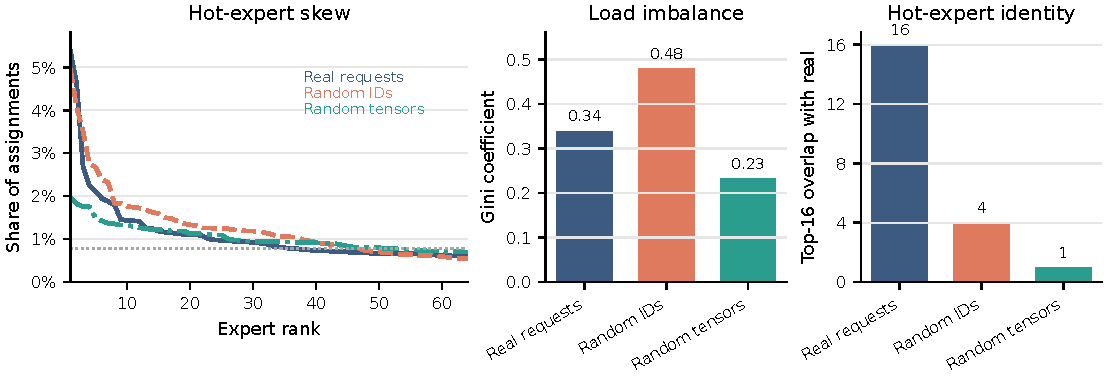
\includegraphics[width=0.7\textwidth]{figures/moe_input_capture.pdf}
\caption{\textbf{Input capture changes data-dependent execution.} First MoE layer of Qwen3-VL-30B-A3B-Instruct-FP8 (128 experts, top-8 routing) under three inputs: real WildChat requests, random token IDs (matched lengths), and random tensors injected at the gate. Random tensors look near-uniform; random tokens skew differently from real requests, with only 4 of the top-16 hot experts in common.}
\label{fig:moe-input-capture}
\end{figure}

Many production operators have data-dependent control flow---which experts, sparse blocks, cache slots, or communication paths execute is determined by the input.
We isolate this effect on a well-known case: the first MoE gate of Qwen3-VL-30B-A3B-Instruct-FP8 (Figure~\ref{fig:moe-input-capture}). Random tensors yield a near-uniform gate (Gini $0.232$); random token IDs over-concentrate load and identify different hot experts from real WildChat requests (Gini $0.480$ vs.\ $0.339$; only $4 / 16$ shared hot experts).
\fastkernels{}'s capture-and-replay path therefore rewards data-dependent kernels on the tensors production requests actually create, rather than on synthetic control flow: the kernel tier can replay golden inputs captured from real end-to-end executions (Appendix~\ref{app:capture}), and the end-to-end tier runs real requests.

\section{Experimental Details}
\label{app:experimental}

\paragraph{Hardware.}
End-to-end L4 validate results in Section~\ref{sec:eval-results} and Tables~\ref{tab:bench_detail}--\ref{tab:bench_detail_b} are measured on a NVIDIA DGX B200 box with 8x NVIDIA B200 SXM GPUs, 180 GB HBM3e each (1.44 TB total), interconnected via 5th-gen NVLink/NVSwitch.
Single-GPU experiments use one GPU; multi-GPU experiments use up to $8\times$B200 (tensor-parallel degree matching the production reference: e.g. TP=2 Mixtral/GPT-OSS, TP=8 GLM-5.2).
L1--L3 agent captures in Section~\ref{sec:eval-agents} use the same B200 nodes.
The Hopper results in Appendix~\ref{app:reference_perf_h200} repeat the same L4 scenario table on a node with 8x NVIDIA H200 SXM GPUs, 141 GB HBM3e each, using the same tensor-parallel degrees; GLM-5.2 is not run there because its NVFP4 kernels require Blackwell.

\paragraph{Serving benchmark.}
Autoregressive L4 throughput uses a mixed-length request mix and a long-context mix against the production server (vLLM, SGLang, or FLA); latency uses single-request (batch 1) and fixed-batch-32 decoding.
Each latency measurement is the median of 5 iterations.
Non-AR models use family-specific public workloads (Parti-prompts, SEED-TTS-Eval, LibriSpeech, COCO val, Food101, MS MARCO, ALOHA, etc.) as listed in Tables~\ref{tab:bench_detail} and \ref{tab:bench_detail_b}.


\clearpage
\section{Reference Performance and Correctness Details}
\label{app:reference_perf}

Table~\ref{tab:bench_detail} and Table~\ref{tab:bench_detail_b} report the B200 L4 validate run for every architecture; Appendix~\ref{app:reference_perf_h200} repeats it on H200.
Figures~\ref{fig:eval-thr-breakdown} and~\ref{fig:eval-lat-breakdown} plot the per-architecture B200 speedups; Figures~\ref{fig:eval-e2e-h200}--\ref{fig:eval-lat-breakdown-h200} are the H200 counterparts (the category-level B200 bars are Figure~\ref{fig:eval-e2e} in the main text).
For each row we list the production reference, the public workload mix, the geometric mean of throughput and latency speedups over that mix, and the alignment metric against the reference.
Autoregressive rows summarize mean prefix-match length and exact-match rate across throughput scenarios; cosine, top-1, box/label, NLL, and pass flags are reported as published by the corresponding harness.
If a model has no latency workload, Lat.\ is ``---''.
Per-row geometric means match the aggregator used in \textsc{MacroEval} (Section~\ref{sec:metrics}) and in Section~\ref{sec:eval-results}.

\subsection{Blackwell (B200) Results}
\label{app:reference_perf_b200}

\begin{table}[H]
      \centering
      \caption{End-to-end B200 validate results for \fastkernels{} architectures (Part I).
      \emph{Thr.} and \emph{Lat.} are geometric-mean speedups versus the named production reference.
      \emph{Correctness} is the harness alignment summary (prefix-match length and exact-match rate for autoregressive models; cosine, top-1, or pass flags otherwise).}
      \label{tab:bench_detail}
      \scriptsize
      \setlength{\tabcolsep}{2.5pt}
      \resizebox{\linewidth}{!}{%
      \begin{tabular}{@{}ll>{\raggedright\arraybackslash}p{1.55cm}>{\raggedright\arraybackslash}p{2.6cm}cc>{\raggedright\arraybackslash}p{2.35cm}@{}}
      \toprule
      \textbf{Category} & \textbf{Architecture} & \textbf{Reference} & \textbf{Workload} & \textbf{Thr.} & \textbf{Lat.} & \textbf{Correctness} \\
      \midrule
      \multirow{7}{*}{Dense \& MoE LLMs}
       & Llama-3.1 & \texttt{vLLM} & WildChat mixed / long-context & $0.95\times$ & $1.02\times$ & prefix 136.3 / EM 28.6\% \\
       & Mixtral & \texttt{vLLM} & WildChat mixed / long-context & $1.06\times$ & $1.00\times$ & prefix 86.3 / EM 12.2\% \\
       & GLM-5.2 (NVFP4) & \texttt{vLLM} & WildChat mixed / long-context & $1.41\times$ & $0.94\times$ & prefix 33.5 / EM 8.9\% \\
       & BitNet 1.58b & \makecell[l]{Microsoft \\ BitNet GPU} & WildChat mixed / long-context & $1.10\times$ & $1.20\times$ & prefix 122.1 / EM 11.0\% \\
       & GPT-OSS (MXFP4) & \texttt{vLLM} & WildChat mixed / long-context & $0.95\times$ & $0.95\times$ & prefix 53.8 / EM 8.2\% \\
       & EAGLE-3 & \texttt{SGLang} & WildChat EAGLE-3 speculative decoding & $0.93\times$ & $1.04\times$ & prefix 160.6 / EM 37.5\% \\
       & Gemma-4 & \texttt{vLLM} & WildChat mixed / long-context & $1.00\times$ & $1.09\times$ & prefix 70.0 / EM 9.6\% \\
      \midrule
      \multirow{9}{*}{\makecell[l]{Linear Attention\\\& New Archs}}
       & Mamba & \texttt{vLLM} & WildChat mixed / long-context & $2.10\times$ & $2.02\times$ & prefix 129.5 / EM 31.9\% \\
       & Mamba2 & \texttt{vLLM} & WildChat mixed / long-context & $0.96\times$ & $0.95\times$ & prefix 203.1 / EM 54.6\% \\
       & RWKV-7 & \texttt{FLA} & mixed / long-context serving & $1.22\times$ & $1.26\times$ & prefix 100.7 / EM 14.8\% \\
       & GLA & \texttt{FLA} & mixed / long-context serving & $1.44\times$ & $1.75\times$ & prefix 262.1 / EM 70.9\% \\
       & RetNet & \texttt{FLA} & mixed / long-context serving & $3.40\times$ & $1.73\times$ & prefix 94.4 / EM 29.9\% \\
       & Qwen-3-Next & \texttt{vLLM} & mixed / long-context serving & $1.21\times$ & $0.99\times$ & prefix 11.7 / EM 1.4\% \\
       & Kimi-Linear & \texttt{vLLM} & mixed / long-context serving & $1.21\times$ & $1.04\times$ & prefix 63.8 / EM 9.2\% \\
       & TTT-E2E & JAX ref. & pretrain + meta forward & $1.95\times$ & $1.95\times$ & token NLL $\Delta$ 0.022 \\
       & Jamba & \texttt{vLLM} & mixed / long-context serving & $0.84\times$ & $1.10\times$ & prefix 91.4 / EM 15.6\% \\
      \midrule
      \multirow{6}{*}{\makecell[l]{Vision / Video /\\Audio}}
       & FLUX.1-Dev & \texttt{vllm-omni} & Parti-prompts; 512 / 1024 & $1.31\times$ & $1.10\times$ & min cos 0.949 \\
       & HunyuanVideo-1.5 & \texttt{vllm-omni} & 480p short / medium T2V & $1.01\times$ & $1.11\times$ & min cos 0.959 \\
       & SDXL & \texttt{diffusers} & Parti-prompts; 512 / 1024 & $1.03\times$ & $1.02\times$ & min cos 0.919 \\
       & SAM3.1 & \texttt{sam3} & image pipeline + video frames & $1.04\times$ & $1.06\times$ & pass / min cos 0.871 \\
       & Whisper & \texttt{vLLM} & LibriSpeech test.clean & $1.07\times$ & $1.03\times$ & prefix 385.9 / EM 63.5\% \\
       & CosyVoice3 & \texttt{vllm-omni} & SEED-TTS-Eval; short / medium / long & $2.30\times$ & $2.34\times$ & mel cos 0.991 \\
      \midrule
      \multirow{7}{*}{\makecell[l]{Multimodal \&\\Encoders}}
       & Qwen2-VL & \texttt{vLLM} & text / image / video & $1.24\times$ & $1.01\times$ & prefix 246.0 / EM 43.9\% \\
       & Qwen3-VL-8B & \texttt{vLLM} & text / image / video & $1.26\times$ & $1.05\times$ & prefix 141.1 / EM 20.2\% \\
       & Qwen3-VL-235B (FP8) & \texttt{vLLM} & text / image / video & $1.59\times$ & $0.95\times$ & prefix 40.1 / EM 2.9\% \\
       & Qwen-2.5-Omni & \texttt{vLLM} & text / image / video / audio & $1.38\times$ & $1.07\times$ & prefix 161.4 / EM 26.9\% \\
       & SigLIP-2 & \texttt{timm} & default-res + high-res & $1.01\times$ & $1.06\times$ & min cos 1.000 \\
       & DINOv3 & \texttt{timm} & default-res + high-res & $0.94\times$ & $0.94\times$ & min cos 1.000 \\
       & SwinV2 & \texttt{timm} & default-res + high-res & $0.94\times$ & $0.91\times$ & min cos 1.000 \\
      \bottomrule
      \end{tabular}%
      }
  \end{table}

  \begin{table}[H]
      \centering
      \caption{End-to-end B200 validate results for \fastkernels{} architectures (Part II).}
      \label{tab:bench_detail_b}
      \scriptsize
      \setlength{\tabcolsep}{2.5pt}
      \resizebox{\linewidth}{!}{%
      \begin{tabular}{@{}ll>{\raggedright\arraybackslash}p{1.55cm}>{\raggedright\arraybackslash}p{2.6cm}cc>{\raggedright\arraybackslash}p{2.35cm}@{}}
      \toprule
      \textbf{Category} & \textbf{Architecture} & \textbf{Reference} & \textbf{Workload} & \textbf{Thr.} & \textbf{Lat.} & \textbf{Correctness} \\
      \midrule
      \multirow{5}{*}{\makecell[l]{Edge \&\\Detection}}
       & MobileNetV4 & \texttt{timm} & default-res + high-res & $1.03\times$ & $1.04\times$ & min cos 1.000 \\
       & ConvNeXtV2 & \texttt{transformers} & Food101 validation & $1.00\times$ & $1.04\times$ & top-1 1.000 \\
       & EfficientNetV2 & \texttt{timm} & Food101 validation & $1.04\times$ & $1.09\times$ & top-1 1.000 \\
       & YOLOv10 & \makecell[l]{THU-MIG/ \\ yolov10} & COCO val detection & $1.14\times$ & $0.94\times$ & box 0.997 / score 1.000 / lbl 100\% \\
       & RTDetrV2 & \texttt{transformers} & COCO val detection & $0.97\times$ & $0.90\times$ & box 0.928 / score 1.000 / lbl 73.4\% \\
      \midrule
      \multirow{6}{*}{\makecell[l]{3D / Robotics /\\Science}}
       & 3DGS & \texttt{gsplat} & deterministic orbit render & $1.00\times$ & $0.99\times$ & pass / RGB cos 1.000 \\
       & InstantNGP & \texttt{pyngp} & fox render & $0.98\times$ & $0.98\times$ & pass / RGBA cos 1.000 \\
       & PointTransformerV3 & PTv3 ref. & ScanObjectNN + batch-8 & $0.98\times$ & $0.99\times$ & feat.\ cos 0.986 (fail) \\
       & OpenFold3 & OpenFold3 ref. & 4 length buckets & $1.01\times$ & $1.02\times$ & align 100\% \\
       & Pi0 & \texttt{OpenPI} & ALOHA 3-cam / 1-cam & $3.09\times$ & $4.17\times$ & pass / action cos 1.000 \\
       & DP3 & \makecell[l]{3D-Diffusion- \\ Policy} & 1-env + batch-8 & $1.13\times$ & $1.13\times$ & min cos 1.000 \\
      \midrule
      \multirow{5}{*}{\makecell[l]{Recommendation\\\& Specialized}}
       & DLRMv2 & \texttt{TorchRec} & Adult Census CTR batch & $1.10\times$ & $1.37\times$ & cosine undefined \\
       & LightGCN & \texttt{PyG} & recommend-batch & $1.02\times$ & $1.04\times$ & pass / cos 1.000 \\
       & BGE-M3 & \texttt{vLLM} & MLDR documents & $2.35\times$ & $0.97\times$ & pass / cos 0.999 \\
       & ColBERTv2 & \texttt{vLLM} & MS MARCO passages & $3.13\times$ & $1.33\times$ & pass / cos 1.000 \\
       & LLaDA & \texttt{Fast-dLLM} & HumanEval Fast-dLLM dual & $0.96\times$ & $0.96\times$ & prefix 168.6 / EM 56.1\% \\
      \midrule
      \multirow{2}{*}{World Models}
       & Oasis & \texttt{open-oasis} & Minecraft clips; 4 DDIM settings & $1.17\times$ & $1.16\times$ & pass / min cos 0.997 \\
       & V-JEPA 2 & \texttt{transformers} & predictor / encoder & $0.97\times$ & $0.98\times$ & pass / cos 1.000 \\
      \bottomrule
      \end{tabular}%
      }

      \vspace{4pt}
      {\small \textit{Note:} Speedup values are geometric means over all validate scenarios for that row; values below $1$ indicate slower execution than the reference.
      CosyVoice3 e2e correctness is the overall median mel-spectrogram cosine from the run log (the compact markdown table left this field blank).
      DLRMv2 reports \texttt{pass=False} with NaN cosine against TorchRec on this checkpoint; PointTransformerV3 reports \texttt{pass=False} at feature cosine $0.986$.
      RetNet's $3.40\times$ throughput geomean still mixes a $6.83\times$ mixed scenario (prefix 21.2) with $1.69\times$ long-context (prefix 167.6).}
  \end{table}

\begin{figure}[H]
  \centering
  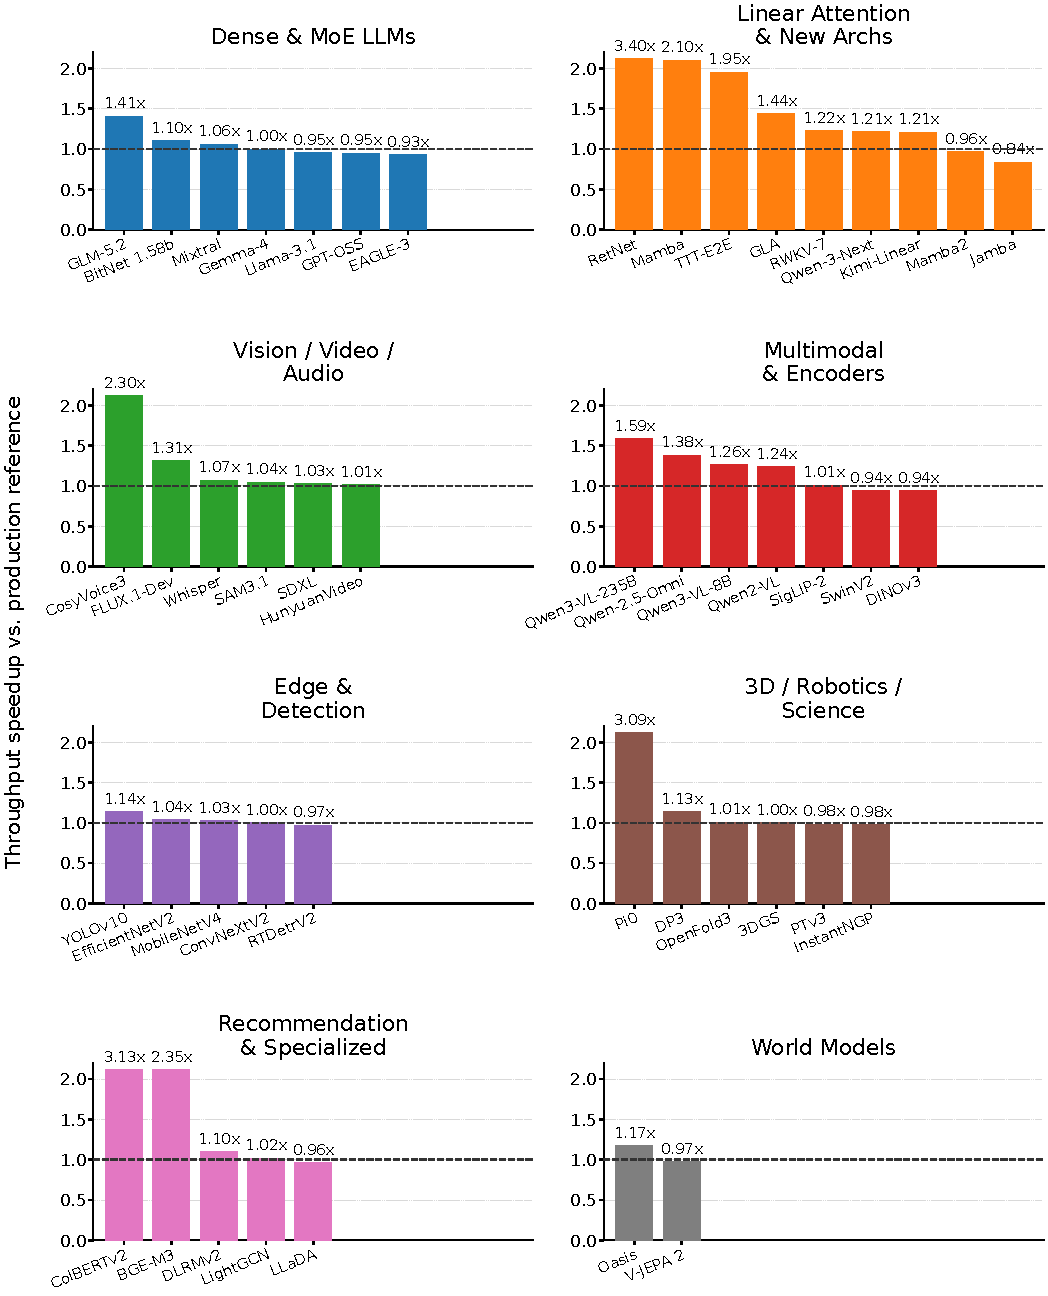
\includegraphics[width=\linewidth]{figures/eval_speedup_breakdown_b200.pdf}
  \caption{\textbf{Per-architecture throughput speedup on B200}, grouped by category. Bars taller than the axis are clipped and labeled with their value; the dashed line marks parity.}
  \label{fig:eval-thr-breakdown}
\end{figure}

\begin{figure}[H]
  \centering
  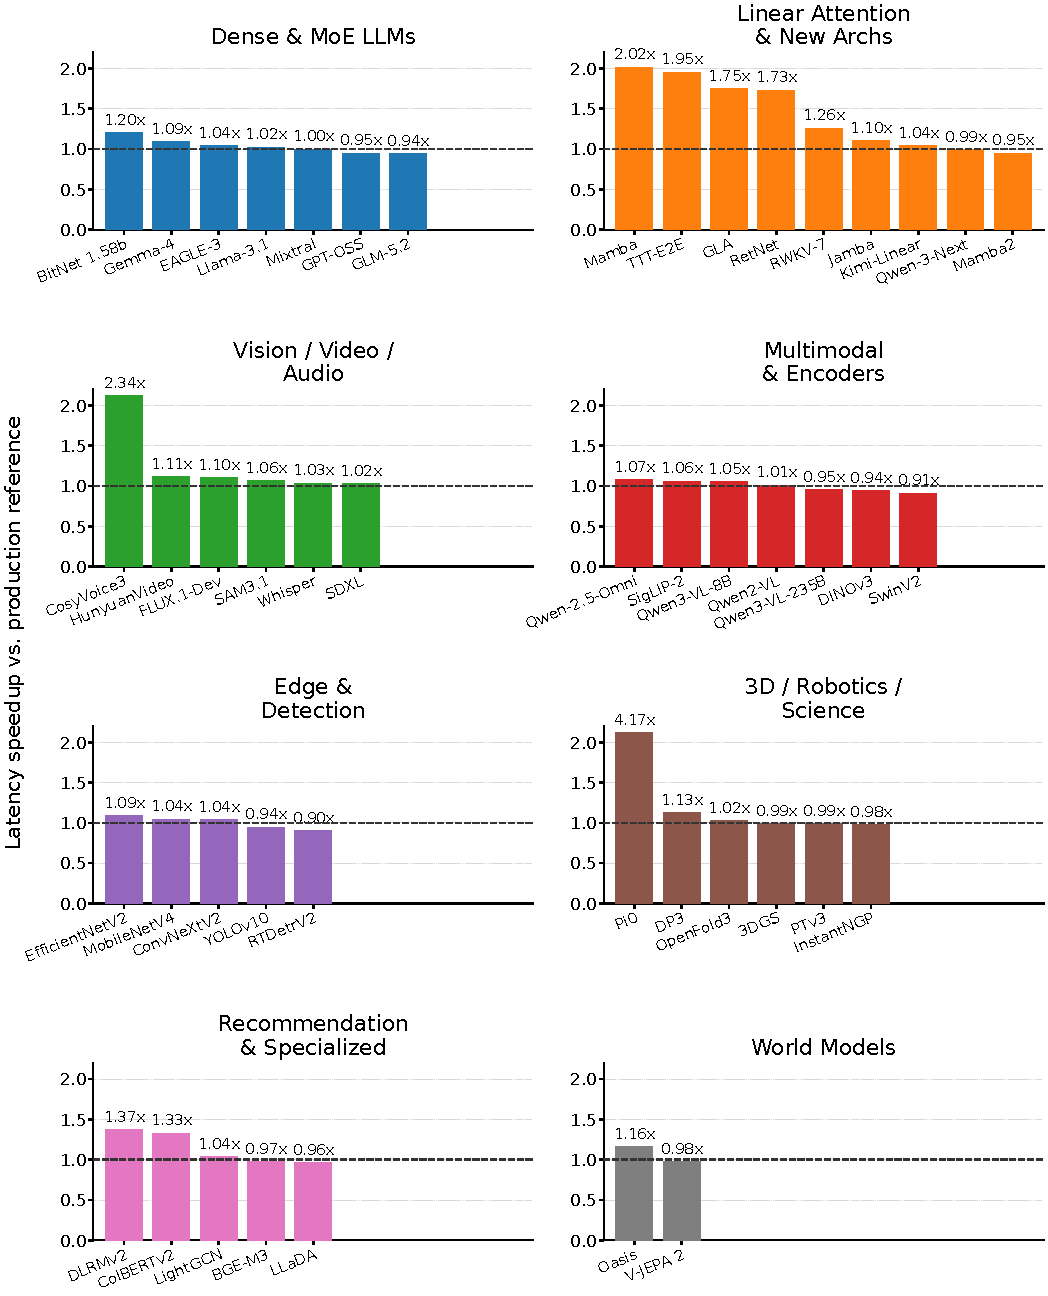
\includegraphics[width=\linewidth]{figures/eval_latency_breakdown_b200.pdf}
  \caption{\textbf{Per-architecture latency speedup on B200}, drawn as in Figure~\ref{fig:eval-thr-breakdown}.}
  \label{fig:eval-lat-breakdown}
\end{figure}

\subsection{Hopper (H200) Results}
\label{app:reference_perf_h200}

Tables~\ref{tab:bench_detail_h200} and~\ref{tab:bench_detail_h200_b} repeat the L4 validate run on $8\times$H200 (Appendix~\ref{app:experimental}) with the same scenario table, workloads, references, and aggregation as the B200 tables above.
Figure~\ref{fig:eval-e2e-h200} is the H200 counterpart of Figure~\ref{fig:eval-e2e}, and Figures~\ref{fig:eval-thr-breakdown-h200} and~\ref{fig:eval-lat-breakdown-h200} are the H200 counterparts of Figures~\ref{fig:eval-thr-breakdown} and~\ref{fig:eval-lat-breakdown}.
Over the 46 architectures that run on both GPUs, the throughput geomean is $1.19\times$ on H200 versus $1.22\times$ on B200, and the latency geomean is $1.15\times$ on both.
The four largest H200 throughput gains (ColBERTv2, RetNet, Pi0, CosyVoice3) are also among the five largest on B200, and dense and MoE LLM serving stays at parity ($0.99\times$); the largest drops relative to B200 are Mamba ($2.10\times \to 1.08\times$) and BGE-M3 ($2.35\times \to 1.37\times$).

\begin{table}[H]
      \centering
      \caption{End-to-end H200 validate results for \fastkernels{} architectures (Part I). Columns as in Table~\ref{tab:bench_detail}.
      $^\dagger$Re-run serially on a second $8\times$H200 node (see the note under Table~\ref{tab:bench_detail_h200_b}).}
      \label{tab:bench_detail_h200}
      \scriptsize
      \setlength{\tabcolsep}{2.5pt}
      \resizebox{\linewidth}{!}{%
      \begin{tabular}{@{}ll>{\raggedright\arraybackslash}p{1.55cm}>{\raggedright\arraybackslash}p{2.6cm}cc>{\raggedright\arraybackslash}p{2.35cm}@{}}
      \toprule
      \textbf{Category} & \textbf{Architecture} & \textbf{Reference} & \textbf{Workload} & \textbf{Thr.} & \textbf{Lat.} & \textbf{Correctness} \\
      \midrule
      \multirow{7}{*}{Dense \& MoE LLMs}
       & Llama-3.1 & \texttt{vLLM} & WildChat mixed / long-context & $0.97\times$ & $1.00\times$ & prefix 140.3 / EM 28.5\% \\
       & Mixtral & \texttt{vLLM} & WildChat mixed / long-context & $1.02\times$ & $1.01\times$ & prefix 72.9 / EM 9.7\% \\
       & GLM-5.2 (NVFP4) & \texttt{vLLM} & WildChat mixed / long-context & --- & --- & not run (NVFP4 is Blackwell-only) \\
       & BitNet 1.58b & \makecell[l]{Microsoft \\ BitNet GPU} & WildChat mixed / long-context & $1.01\times$ & $1.10\times$ & prefix 108.2 / EM 7.8\% \\
       & GPT-OSS (MXFP4) & \texttt{vLLM} & WildChat mixed / long-context & $1.04\times$ & $0.92\times$ & prefix 63.0 / EM 8.8\% \\
       & EAGLE-3$^\dagger$ & \texttt{SGLang} & WildChat EAGLE-3 speculative decoding & $0.96\times$ & $1.04\times$ & prefix 179.2 / EM 50.0\% \\
       & Gemma-4 & \texttt{vLLM} & WildChat mixed / long-context & $0.92\times$ & $1.03\times$ & prefix 72.3 / EM 7.3\% \\
      \midrule
      \multirow{9}{*}{\makecell[l]{Linear Attention\\\& New Archs}}
       & Mamba & \texttt{vLLM} & WildChat mixed / long-context & $1.08\times$ & $1.03\times$ & prefix 147.7 / EM 36.9\% \\
       & Mamba2 & \texttt{vLLM} & WildChat mixed / long-context & $0.99\times$ & $0.96\times$ & prefix 207.1 / EM 53.5\% \\
       & RWKV-7 & \texttt{FLA} & mixed / long-context serving & $1.34\times$ & $1.29\times$ & prefix 99.8 / EM 12.7\% \\
       & GLA & \texttt{FLA} & mixed / long-context serving & $1.34\times$ & $1.67\times$ & prefix 264.1 / EM 71.1\% \\
       & RetNet & \texttt{FLA} & mixed / long-context serving & $3.05\times$ & $1.75\times$ & prefix 98.8 / EM 32.2\% \\
       & Qwen-3-Next & \texttt{vLLM} & mixed / long-context serving & $1.02\times$ & $0.99\times$ & prefix 11.4 / EM 1.3\% \\
       & Kimi-Linear & \texttt{vLLM} & mixed / long-context serving & $1.07\times$ & $0.89\times$ & prefix 18.3 / EM 4.0\% \\
       & TTT-E2E & JAX ref. & pretrain + meta forward & $1.75\times$ & $1.75\times$ & token NLL $\Delta$ 0.022 \\
       & Jamba$^\dagger$ & \texttt{vLLM} & mixed / long-context serving & $0.96\times$ & $1.06\times$ & prefix 98.3 / EM 16.4\% \\
      \midrule
      \multirow{6}{*}{\makecell[l]{Vision / Video /\\Audio}}
       & FLUX.1-Dev & \texttt{vllm-omni} & Parti-prompts; 512 / 1024 & $1.11\times$ & $1.02\times$ & min cos 0.981 \\
       & HunyuanVideo-1.5 & \texttt{vllm-omni} & 480p short / medium T2V & $1.00\times$ & $1.10\times$ & min cos 0.943 \\
       & SDXL & \texttt{diffusers} & Parti-prompts; 512 / 1024 & $1.01\times$ & $1.02\times$ & min cos 0.923 \\
       & SAM3.1 & \texttt{sam3} & image pipeline + video frames & $1.13\times$ & $1.10\times$ & pass / min cos 0.871 \\
       & Whisper & \texttt{vLLM} & LibriSpeech test.clean & $1.04\times$ & $0.95\times$ & prefix 386.1 / EM 63.6\% \\
       & CosyVoice3 & \texttt{vllm-omni} & SEED-TTS-Eval; short / medium / long & $2.85\times$ & $2.05\times$ & mel cos 0.991 \\
      \midrule
      \multirow{7}{*}{\makecell[l]{Multimodal \&\\Encoders}}
       & Qwen2-VL & \texttt{vLLM} & text / image / video & $1.13\times$ & $0.99\times$ & prefix 248.2 / EM 44.8\% \\
       & Qwen3-VL-8B & \texttt{vLLM} & text / image / video & $1.21\times$ & $1.02\times$ & prefix 139.5 / EM 19.9\% \\
       & Qwen3-VL-235B (FP8) & \texttt{vLLM} & text / image / video & $1.56\times$ & $0.98\times$ & prefix 41.9 / EM 2.8\% \\
       & Qwen-2.5-Omni & \texttt{vLLM} & text / image / video / audio & $1.43\times$ & $1.01\times$ & prefix 158.9 / EM 25.0\% \\
       & SigLIP-2$^\dagger$ & \texttt{timm} & default-res + high-res & $1.00\times$ & $1.06\times$ & min cos 0.986 \\
       & DINOv3$^\dagger$ & \texttt{timm} & default-res + high-res & $0.94\times$ & $0.89\times$ & min cos 1.000 \\
       & SwinV2$^\dagger$ & \texttt{timm} & default-res + high-res & $1.00\times$ & $1.04\times$ & min cos 1.000 \\
      \bottomrule
      \end{tabular}%
      }
  \end{table}

  \begin{table}[H]
      \centering
      \caption{End-to-end H200 validate results for \fastkernels{} architectures (Part II).}
      \label{tab:bench_detail_h200_b}
      \scriptsize
      \setlength{\tabcolsep}{2.5pt}
      \resizebox{\linewidth}{!}{%
      \begin{tabular}{@{}ll>{\raggedright\arraybackslash}p{1.55cm}>{\raggedright\arraybackslash}p{2.6cm}cc>{\raggedright\arraybackslash}p{2.35cm}@{}}
      \toprule
      \textbf{Category} & \textbf{Architecture} & \textbf{Reference} & \textbf{Workload} & \textbf{Thr.} & \textbf{Lat.} & \textbf{Correctness} \\
      \midrule
      \multirow{5}{*}{\makecell[l]{Edge \&\\Detection}}
       & MobileNetV4$^\dagger$ & \texttt{timm} & default-res + high-res & $1.04\times$ & $1.11\times$ & min cos 1.000 \\
       & ConvNeXtV2 & \texttt{transformers} & Food101 validation & $1.00\times$ & $0.99\times$ & top-1 1.000 \\
       & EfficientNetV2 & \texttt{timm} & Food101 validation & $1.06\times$ & $0.99\times$ & top-1 1.000 \\
       & YOLOv10 & \makecell[l]{THU-MIG/ \\ yolov10} & COCO val detection & $1.04\times$ & $2.61\times$ & box 0.461 / score 0.549 / lbl 94.6\% (fail) \\
       & RTDetrV2 & \texttt{transformers} & COCO val detection & $1.00\times$ & $0.85\times$ & box 0.928 / score 1.000 / lbl 73.4\% \\
      \midrule
      \multirow{6}{*}{\makecell[l]{3D / Robotics /\\Science}}
       & 3DGS & \texttt{gsplat} & deterministic orbit render & $1.00\times$ & $1.00\times$ & pass / RGB cos 1.000 \\
       & InstantNGP & \texttt{pyngp} & fox render & $0.99\times$ & $0.99\times$ & pass / RGBA cos 1.000 \\
       & PointTransformerV3 & PTv3 ref. & ScanObjectNN + batch-8 & $1.00\times$ & $0.99\times$ & feat.\ cos 0.986 (fail) \\
       & OpenFold3 & OpenFold3 ref. & 4 length buckets & $1.00\times$ & $0.95\times$ & align 100\% \\
       & Pi0 & \texttt{OpenPI} & ALOHA 3-cam / 1-cam & $2.98\times$ & $3.71\times$ & pass / action cos 1.000 \\
       & DP3 & \makecell[l]{3D-Diffusion- \\ Policy} & 1-env + batch-8 & $1.14\times$ & $1.17\times$ & min cos 1.000 \\
      \midrule
      \multirow{5}{*}{\makecell[l]{Recommendation\\\& Specialized}}
       & DLRMv2 & \texttt{TorchRec} & Adult Census CTR batch & $1.07\times$ & $1.34\times$ & cosine undefined \\
       & LightGCN & \texttt{PyG} & recommend-batch & $1.02\times$ & $1.04\times$ & pass / cos 1.000 \\
       & BGE-M3 & \texttt{vLLM} & MLDR documents & $1.37\times$ & $1.04\times$ & pass / cos 0.997 \\
       & ColBERTv2 & \texttt{vLLM} & MS MARCO passages & $3.77\times$ & $2.59\times$ & pass / cos 1.000 \\
       & LLaDA & \texttt{Fast-dLLM} & HumanEval Fast-dLLM dual & $1.04\times$ & $1.05\times$ & prefix 166.2 / EM 53.7\% \\
      \midrule
      \multirow{2}{*}{World Models}
       & Oasis & \texttt{open-oasis} & Minecraft clips; 4 DDIM settings & $1.17\times$ & $1.13\times$ & pass / min cos 0.996 \\
       & V-JEPA 2 & \texttt{transformers} & predictor / encoder & $0.99\times$ & $1.00\times$ & pass / cos 1.000 \\
      \bottomrule
      \end{tabular}%
      }

      \vspace{4pt}
      {\small \textit{Note:} Aggregation as in Tables~\ref{tab:bench_detail}--\ref{tab:bench_detail_b}.
      $^\dagger$EAGLE-3, Jamba, and the four \texttt{timm} encoders failed in the parallel run for environment reasons (an SGLang~0.5.20 \texttt{ServerArgs} API change, a CUDA illegal-memory-access crash that did not reproduce, and gated ImageNet access, respectively) and were re-run serially on a second $8\times$H200 node with the same software stack; the EAGLE-3 re-run also needed a two-line compatibility fix in the SGLang harness.
      YOLOv10 fails alignment on H200 (box cosine $0.461$ vs.\ $0.997$ on B200), so its H200 speedups, notably the $2.61\times$ latency, are not like-for-like and should not be read as gains.
      DLRMv2 again reports a degenerate cosine ($0$ here, NaN on B200) with a maximum absolute difference of $0$; PointTransformerV3 fails at feature cosine $0.986$ as on B200.
      RetNet's $3.05\times$ throughput geomean mixes a $5.61\times$ mixed scenario (prefix 19.1) with $1.66\times$ long-context (prefix 178.4).}
  \end{table}

\begin{figure}[H]
  \centering
  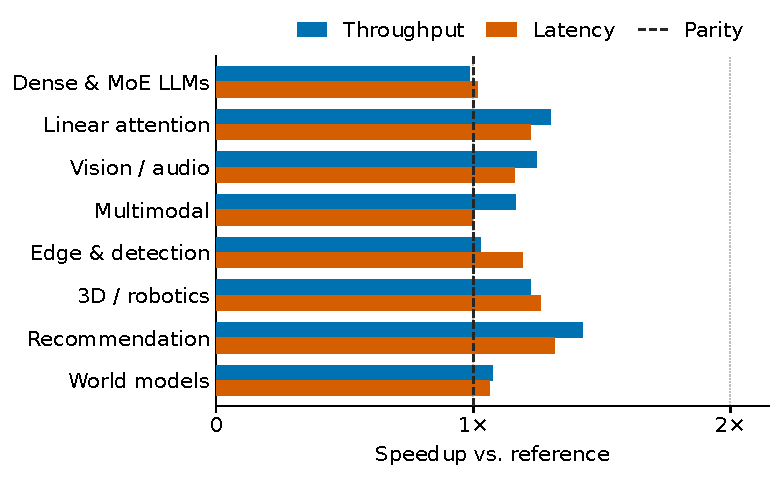
\includegraphics[width=0.7\linewidth]{figures/eval_e2e_h200.pdf}
  \caption{\textbf{End-to-end speedup by category on H200.}
  Counterpart of Figure~\ref{fig:eval-e2e}: each bar is the geometric mean over the architectures of that category in Tables~\ref{tab:bench_detail_h200} and~\ref{tab:bench_detail_h200_b} (GLM-5.2 is not run).
  The edge \& detection latency bar includes YOLOv10, which fails alignment on H200; without it, that bar is $0.98\times$.}
  \label{fig:eval-e2e-h200}
\end{figure}

\begin{figure}[H]
  \centering
  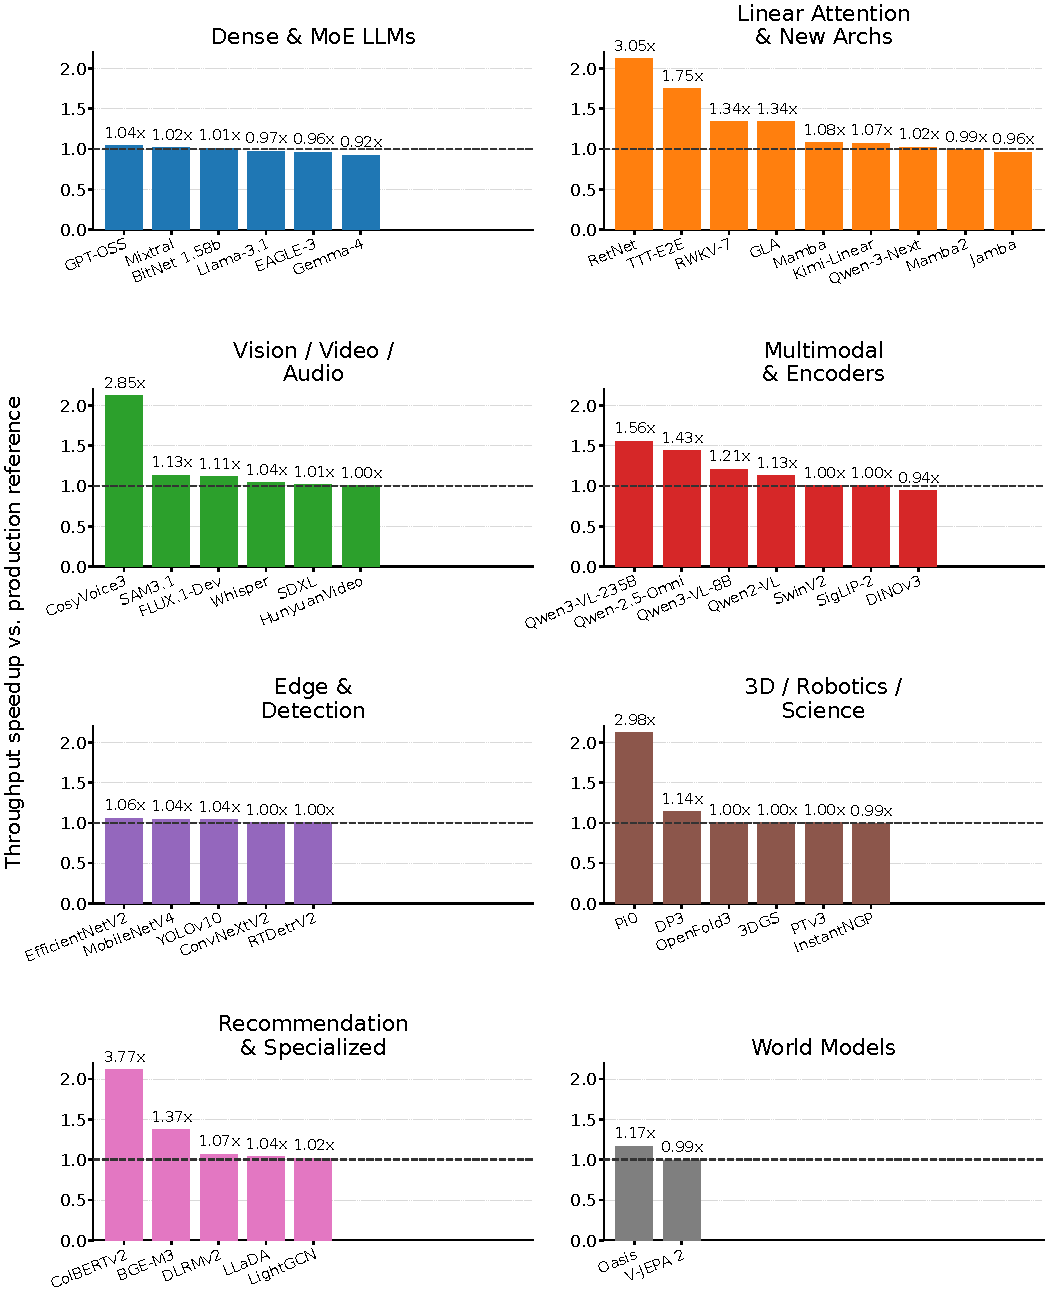
\includegraphics[width=\linewidth]{figures/eval_speedup_breakdown_h200.pdf}
  \caption{\textbf{Per-architecture throughput speedup on H200}, grouped by category. Bars taller than the axis are clipped and labeled with their value; the dashed line marks parity.}
  \label{fig:eval-thr-breakdown-h200}
\end{figure}

\begin{figure}[H]
  \centering
  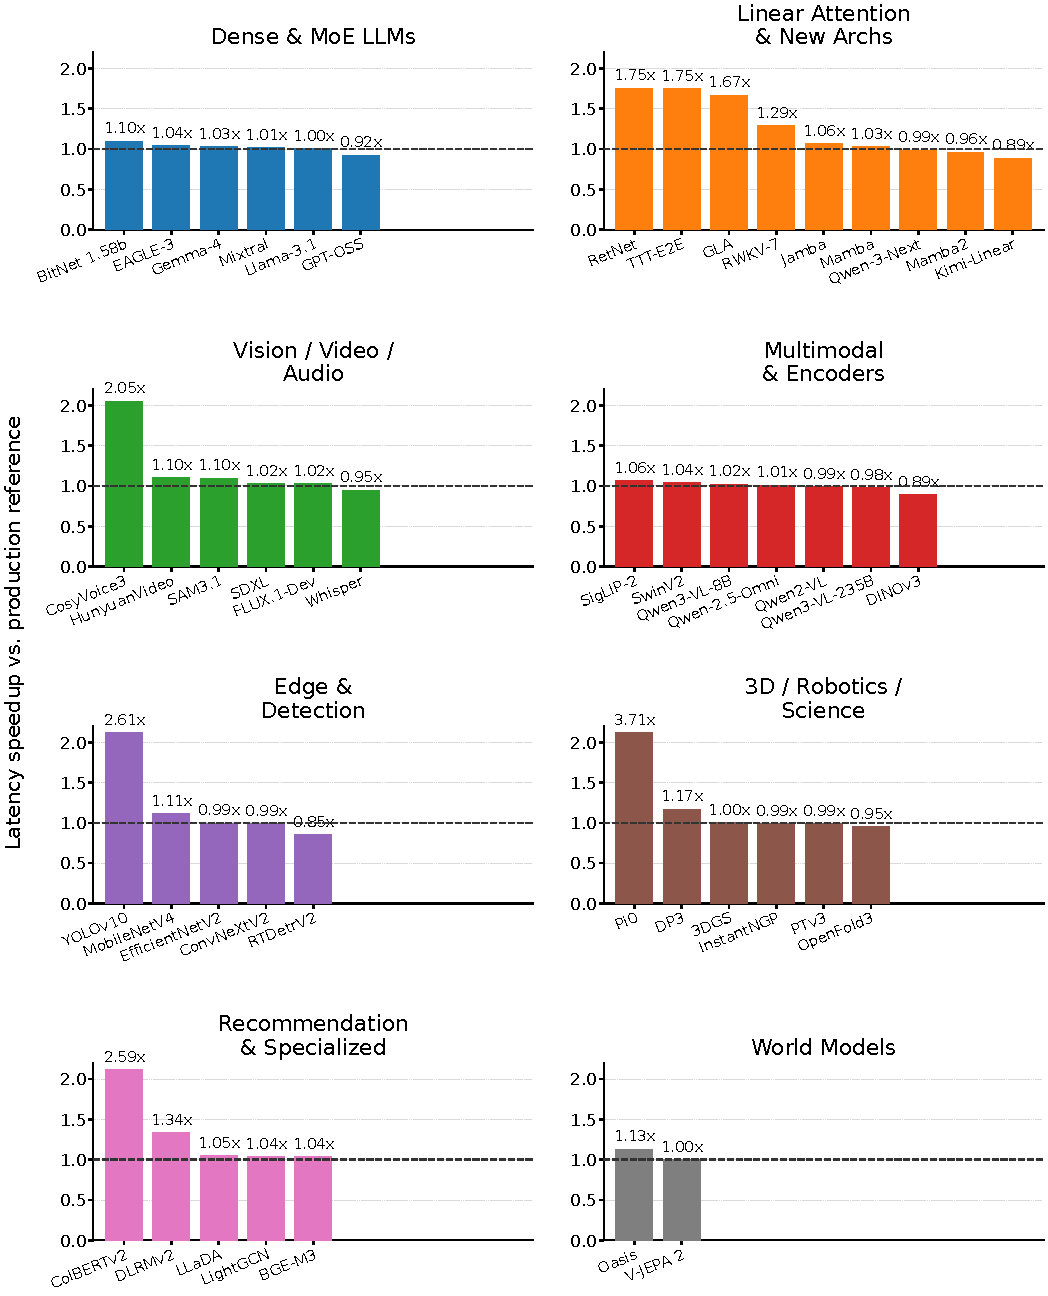
\includegraphics[width=\linewidth]{figures/eval_latency_breakdown_h200.pdf}
  \caption{\textbf{Per-architecture latency speedup on H200}, drawn as in Figure~\ref{fig:eval-thr-breakdown-h200}. YOLOv10's $2.61\times$ comes from a run that fails alignment (Table~\ref{tab:bench_detail_h200_b}).}
  \label{fig:eval-lat-breakdown-h200}
\end{figure}


\section{Baseline Versioning and Drift}
\label{app:drift}

Production kernels are a moving target, so \fastkernels{} is versioned: each release pins the exact revision of every reference library (vLLM, FlashInfer, FLA, diffusers, \dots) per target GPU, and the results in this paper use vLLM~0.26.0 (released 2026-07-25).
A speedup over a \fastkernels{} baseline is therefore a speedup over production at that release.
To track drift, \fastkernels{} ships a daily CI job (\texttt{scripts/baseline\_drift.sh}): whenever a new vLLM release appears, it re-benchmarks only the reference models under that release on each pinned GPU type, in isolated environments with one job per node, and computes per-family drift coefficients (per-model geometric mean over workloads, models weighted equally within a family).
Dividing a speedup measured against the pinned baseline by the family coefficient estimates the speedup against the newer release; when any family moves by more than 10\%, a re-release with re-pinned references is prepared.

To estimate the cadence this implies, we ran the same measurement over the 127 days between vLLM~0.18.0 (2026-03-20) and 0.26.0 on 8$\times$H200 and 8$\times$B200, on the 13 reference models both releases serve, with identical workloads (Table~\ref{tab:drift}).
The median model moved by only $1.03\times$ (throughput) and $1.01\times$ (latency) on H200, and by $1.07\times$ and $1.09\times$ on B200.
Drift is concentrated rather than uniform: one family crossed the 10\% threshold on H200 (linear attention and SSMs, $1.15\times$ throughput) and two on B200, where the LLM family is dominated by gpt-oss-120b's MXFP4 path maturing on Blackwell ($2.8\times$, against $1.04\times$ on H200).
Newer releases are not uniformly faster: Qwen3-VL-235B-FP8 lost throughput on both GPUs ($0.83\times$ and $0.87\times$).
This implies a re-release at least every four months, sooner on newer hardware whose support for new number formats is still maturing---comparable to the cadence at which any benchmark that stays current must add newly released architectures.

\begin{table}[H]
  \centering
  \caption{\textbf{Reference drift from vLLM~0.18.0 to 0.26.0} (127 days), as computed by the baseline-drift CI job: speedup of the newer release (${>}1$: faster), per-model geometric mean over workloads, models weighted equally within a family.
  Latencies are 5-iteration medians (${<}1\%$ spread); throughput is one timed pass per workload, which three repeated runs per release of Qwen3-VL-235B-FP8 place within 1.5\%.
  On B200, six models needed \texttt{nvidia-cutlass-dsl==4.5.3} to import under vLLM~0.18.0.}
  \label{tab:drift}
  \small
  % Generated by figures/make_drift_table.py. Do not edit by hand.
\begin{tabular}{@{}lr rr rr@{}}
\toprule
 & & \multicolumn{2}{c}{\textbf{H200}} & \multicolumn{2}{c}{\textbf{B200}} \\
\cmidrule(lr){3-4}\cmidrule(lr){5-6}
Model family & $n$ & Thr. & Lat. & Thr. & Lat. \\
\midrule
LLM (dense + MoE) & 3 & 1.09$\times$ & 1.08$\times$ & 1.44$\times$ & 1.37$\times$ \\
Linear attention / SSM / hybrid & 5 & 1.15$\times$ & 1.03$\times$ & 1.14$\times$ & 1.18$\times$ \\
Multimodal / VLM & 4 & 0.98$\times$ & 1.05$\times$ & 1.01$\times$ & 1.07$\times$ \\
Audio & 1 & 1.02$\times$ & 1.02$\times$ & 1.02$\times$ & 1.07$\times$ \\
\midrule
Median model & 13 & 1.03$\times$ & 1.01$\times$ & 1.07$\times$ & 1.09$\times$ \\
\bottomrule
\end{tabular}

\end{table}

\section{Agent Selection, Configuration, and Cost}
\label{app:agents}

\paragraph{Selection.}
We chose agents to cover the three lines of work that currently produce the strongest kernels.
From the KernelBench ecosystem we run Dr.~Kernel~\citep{drkernel}, one of its most recent agents; of the others we tried, KernelAgent~\citep{kernelagent} did not reproduce its reported results in our setting, and the rest assume KernelBench's single-file tasks with a self-contained reference and cannot load production-shaped modules that require configuration objects, KV-cache wrappers, packed quantized weights, or a distributed context.
From the MLSys 2026 FlashInfer AI Kernel Generation Contest~\citep{mlsys26contest}, whose tasks were drawn from production LLM workloads and scored against FlashInfer's expert kernels, we run KDA~\citep{kda}, whose full-agent entry placed first on MoE, second on DSA, and third on GDN, and AKO~\citep{ako} (its AKO4X harness was adapted by the GEMM People entry, which placed second on MoE), whose release reports beating the FlashInfer expert kernels on 9 of 10 operator families on B200.
Finally, we run Claude Code and Codex~\citep{codex} directly, with no harness.
Because KDA and AKO drive the same Claude model as our Claude Code runs (KDA adds a GPT reviewer), comparing them with Claude Code isolates the contribution of the harness.

\paragraph{Configurations.}
Table~\ref{tab:agent-config} summarizes how each agent was run.
All agents receive the same task: the baseline module, its captured cases, and \texttt{fastkernels bench} on a GPU that is leased only while they benchmark or profile.
A candidate becomes a \emph{winner} only if every non-skipped case passes and its geometric-mean speedup is at least $1\times$; an unchanged baseline that passes counts as correct at $1\times$ but not as a fast$_1$ win.
The independent campaign optimizes all 133 operators in standalone mode; the sequential campaign regenerates the 86 L2 and L3 operators on top of the frozen lower-level winners.

\begin{table}[H]
  \centering
  \caption{\textbf{Agent configurations.} \emph{Cap}: hang cap on one agent session (the candidate is kept on timeout), not a target budget.}
  \label{tab:agent-config}
  \scriptsize
  \setlength{\tabcolsep}{3pt}
  \begin{tabular}{@{}l>{\raggedright\arraybackslash}p{3.4cm}>{\raggedright\arraybackslash}p{6.2cm}l@{}}
  \toprule
  \textbf{Agent} & \textbf{Model(s)} & \textbf{Loop per operator} & \textbf{Cap} \\
  \midrule
  Dr.~Kernel & released \texttt{drkernel-14b} & 8 samples $\times$ 3 generate--execute--feedback turns (temperature 1.0, top-$p$ 0.95) & --- \\
  Claude Code & Claude Opus 5 (1M context, high effort) & one session with the default tools & 5\,h \\
  Codex & GPT-5.6 sol (high) & one session, same prompt as Claude Code & 5\,h \\
  KDA & Claude Opus 5 (draft, plan, implement); GPT-5.6 sol (review) & one planning cycle, then two implement--review rounds, with KernelWiki and Nsight Compute skills & 6\,h \\
  AKO & Claude Opus 5 (master and sub-agents) & two master-directed rounds, each a fresh sub-agent rewriting the kernel along one direction; improving kernels are archived & 5\,h/round \\
  \bottomrule
  \end{tabular}
\end{table}

\paragraph{Budget and the number of agents.}
Table~\ref{tab:agent-cost} reports what each agent spent: 6{,}914 agent-hours and 41.9B tokens (266M output tokens) in total, of which Claude Code, KDA, and AKO account for 1{,}763, 2{,}512, and 2{,}234 agent-hours.
These are the budgets at which such agents are used in practice: the MLSys 2026 contest gave teams 13 weeks, from the release of the starter kit (January 22) to the kernel deadline (April 24), to optimize five kernels~\citep{mlsys26contest}.
A leaderboard that samples many models for a few turns per task is far cheaper per entry, but it measures a different system than the long-horizon agents practitioners deploy, and the ranking of those agents is what \fastkernels{} is meant to report.
Each additional long-horizon agent costs about 2{,}000 agent-hours and 8--22B tokens on the default set.
Codex is the exception worth noting: its kernel-level results are comparable to the Claude-based agents' at 321 agent-hours.
\fastkernels{} imposes no structure on the agent, so any agent that writes candidate files can be scored with the same harness.

\paragraph{Evolutionary search.}
AlphaEvolve~\citep{alphaevolve} and KernelEvolve~\citep{kernelevolve} are not publicly available.
OpenEvolve~\citep{openevolve} is, and was the organizers' agent baseline in the MLSys 2026 contest, but evolutionary frameworks evaluate a population of candidates in every generation, and on \fastkernels{} each evaluation compiles a kernel and benchmarks it on its production-shaped cases (for collectives, on a full tensor-parallel group); their cost per operator therefore scales with population size times the number of generations, on top of the LLM calls that produce each candidate, which puts a 133-operator campaign beyond our budget.
The AKO authors also report that, during the contest, search-based methods performed far worse than letting a coding agent optimize kernels directly~\citep{ako}.

\begin{table}[H]
  \centering
  \caption{\textbf{Agent cost per campaign} (133 operators independently, 86 regenerated sequentially).
  \emph{Agent-hours}: sum over operators of each operator's wall-clock generation time, including relaunches; operators run in parallel, so this is not campaign wall-clock time.
  \emph{Tokens} as reported by each agent's CLI or API: input, output, and cached (re-read) context; output includes reasoning tokens.
  Dr.~Kernel runs a local model without prompt caching; KDA counts both its Claude and Codex sessions.}
  \label{tab:agent-cost}
  \small
  \setlength{\tabcolsep}{4pt}
  % Generated by figures/make_agent_cost.py. Do not edit by hand.
\begin{tabular}{@{}ll r rr rrr@{}}
\toprule
 & & & \multicolumn{2}{c}{\textbf{Agent-hours}} & \multicolumn{3}{c}{\textbf{Tokens}} \\
\cmidrule(lr){4-5}\cmidrule(lr){6-8}
Agent & Campaign & Ops & Total & Median/op & Total (B) & Output (M) & Cached (\%) \\
\midrule
\multirow{2}{*}{Dr.~Kernel} & Independent & 133 & 53 & 0.26 & 0.03 & 10.4 & --- \\
 & Sequential & 86 & 32 & 0.34 & 0.02 & 8.0 & --- \\
\midrule
\multirow{2}{*}{Claude Code} & Independent & 133 & 1,171 & 7.27 & 4.35 & 31.4 & 97 \\
 & Sequential & 86 & 592 & 6.06 & 3.58 & 22.5 & 97 \\
\midrule
\multirow{2}{*}{KDA} & Independent & 133 & 1,751 & 12.33 & 12.31 & 62.8 & 96 \\
 & Sequential & 86 & 762 & 8.22 & 9.48 & 42.2 & 97 \\
\midrule
\multirow{2}{*}{AKO} & Independent & 133 & 1,421 & 9.43 & 5.47 & 47.4 & 97 \\
 & Sequential & 86 & 813 & 8.70 & 4.86 & 35.3 & 97 \\
\midrule
\multirow{2}{*}{Codex} & Independent & 133 & 253 & 1.86 & 1.02 & 4.0 & 98 \\
 & Sequential & 86 & 67 & 0.71 & 0.74 & 2.4 & 98 \\
\bottomrule
\end{tabular}

\end{table}

\section{Additional Kernel-Level Results}
\label{app:fastp}

Figure~\ref{fig:kernel-fastp} extends the fast$_1$ and fast$_2$ columns of Table~\ref{tab:kernel-levels} to every speedup threshold $p$, for the independent mode.

\begin{figure}[H]
  \centering
  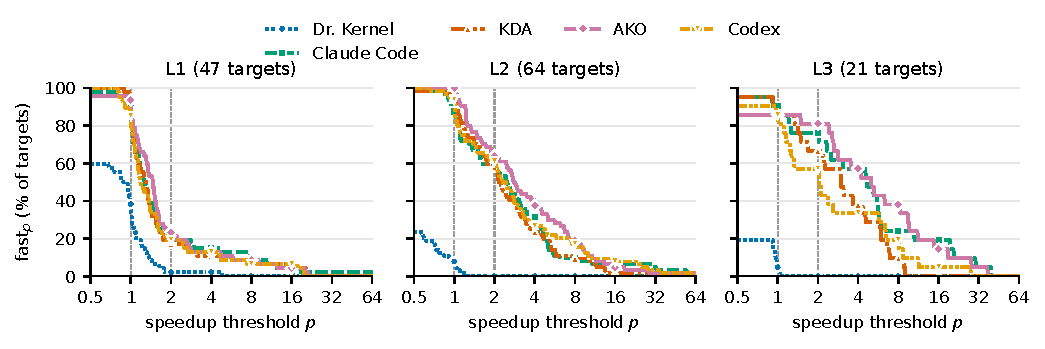
\includegraphics[width=\linewidth]{figures/kernel_fastp.pdf}
  \caption{\textbf{fast$_p$ by level (independent mode).} Share of targets whose kernel is correct and more than $p\times$ faster than the production baseline; the value at the left edge approaches the share of correct kernels. Dashed lines mark $p=1$ and $p=2$.}
  \label{fig:kernel-fastp}
\end{figure}

Table~\ref{tab:kernel-composition} compares the same operators across the three kernel-bench modes (Section~\ref{sec:eval-agents}).

\begin{table}[H]
  \centering
  \caption{\textbf{Composition effect and sequential generation}, over operators correct in both modes ($n$).
  \emph{Ratio}: geometric mean of the per-operator speedup ratio (composed / independent, or sequential / composed).
  \emph{Broke}: independent winners that fail correctness once composed.}
  \label{tab:kernel-composition}
  \small
  \setlength{\tabcolsep}{3pt}
  \begin{tabular}{@{}l rrr rrr rr rr@{}}
\toprule
 & \multicolumn{6}{c}{\makecell{\textbf{Composition effect}\\(Independent $\to$ Composed)}} & \multicolumn{4}{c}{\makecell{\textbf{Sequential}\\(Composed $\to$ Seq.)}} \\
\cmidrule(lr){2-7}\cmidrule(lr){8-11}
 & \multicolumn{3}{c}{L2} & \multicolumn{3}{c}{L3} & \multicolumn{2}{c}{L2} & \multicolumn{2}{c}{L3} \\
\cmidrule(lr){2-4}\cmidrule(lr){5-7}\cmidrule(lr){8-9}\cmidrule(lr){10-11}
Agent & $n$ & Ratio & Broke & $n$ & Ratio & Broke & $n$ & Ratio & $n$ & Ratio \\
\midrule
Dr.~Kernel & 5 & 0.99$\times$ & 0 & 1 & 1.00$\times$ & 0 & 1 & 1.78$\times$ & 0 & --- \\
Claude Code & 54 & 1.09$\times$ & 2 & 14 & 0.99$\times$ & 4 & 50 & 0.99$\times$ & 14 & 0.97$\times$ \\
KDA & 51 & 0.98$\times$ & 10 & 11 & 0.88$\times$ & 6 & 47 & 0.90$\times$ & 11 & 1.07$\times$ \\
AKO & 60 & 1.00$\times$ & 4 & 14 & 0.86$\times$ & 3 & 55 & 1.05$\times$ & 14 & 1.48$\times$ \\
Codex & 47 & 0.97$\times$ & 13 & 5 & 1.04$\times$ & 13 & 43 & 0.94$\times$ & 5 & 1.35$\times$ \\
\bottomrule
\end{tabular}

\end{table}

\section{End-to-End Results per Model}
\label{app:e2e}

Qwen3-VL-235B uses 200 requests per throughput workload and 32 correctness samples; GLA and OpenFold3 were re-run on cloud B200 nodes after a harness fix, and Codex's sets on a separate B200 node (its Llama baseline throughput is within 0.02\% of the other node's). Every set's speedups and discrepancies are relative to the baseline measured in the same run.
OpenFold3 runs eagerly and deterministically, so its noise run reproduces the reference bit for bit while its diffusion sampling amplifies any numerical change; its $g_i$ therefore comes from a calibration run that instead disables cuBLAS reduced-precision bf16 reductions, a benign numerical change.
Table~\ref{tab:e2e-drops} counts the kernels each set requests and keeps across models, and why kernels were dropped; \emph{Ind.\,+\,Seq.} pools an agent's two sets.
Table~\ref{tab:e2e-per-model} lists, for every model and agent set, the outcome of the all-winners run and of the deployable subset, the number of dropped kernels, the throughput and latency speedups and the mean correctness discrepancy $\bar d$, next to the model's noise floor ($\bar d$ of the noise run and the calibrated $g_i$).
Table~\ref{tab:e2e-sensitivity} reports the agent ranking under $0.5\times$--$2\times$ scaling of the correctness thresholds $g_i$ and $f_i$.

\begin{table}[H]
  \centering
  \caption{\textbf{Why kernel-level winners are dropped end to end.} Kernels are counted per (model, kernel) pair.
  Causes: \emph{Comp.}: breaks the compilation stack (not traceable by \texttt{torch.compile}, or breaks dynamic shapes); \emph{Run.}: crashes at run time on real engine shapes; \emph{T/O}: hangs; \emph{Imp.}: fails to import; \emph{Inc.}: runs but produces wrong outputs.
  \emph{AW crash / broken}: models where the full winner set crashes / runs with wrong outputs; \emph{Not conv.}: no deployable subset found within the attempt budget.}
  \label{tab:e2e-drops}
  \small
  \setlength{\tabcolsep}{3pt}
  \resizebox{\linewidth}{!}{% Generated by figures/make_macroeval.py (11/11 scenarios with a baseline, universe=all: 11 items, 8 families). Do not edit by hand.
\begin{tabular}{@{}ll rr rrrrr rrrrr@{}}
\toprule
 & & \multicolumn{2}{c}{\textbf{Kernels}} & \multicolumn{5}{c}{\textbf{Dropped, by cause}} & \multicolumn{5}{c}{\textbf{Models}} \\
\cmidrule(lr){3-4}\cmidrule(lr){5-9}\cmidrule(lr){10-14}
Agent & Mode & Req. & Kept & Comp. & Run. & T/O & Imp. & Inc. & \makecell{AW\\crash} & \makecell{AW\\broken} & Empty & \makecell{Not\\conv.} & N/A \\
\midrule
\multirow{3}{*}{Dr.~Kernel} & Independent & 53 & 31 & 6 & 7 & 0 & 0 & 4 & 6 & 3 & 0 & 1 & 0 \\
 & Sequential & 54 & 25 & 6 & 7 & 0 & 0 & 5 & 6 & 3 & 0 & 2 & 0 \\
 & Ind.\,+\,Seq. & 107 & 56 & 12 & 14 & 0 & 0 & 9 & 12 & 6 & 0 & 3 & 0 \\
\midrule
\multirow{3}{*}{Claude Code} & Independent & 175 & 85 & 11 & 11 & 1 & 0 & 2 & 6 & 3 & 0 & 4 & 0 \\
 & Sequential & 190 & 93 & 12 & 8 & 1 & 0 & 3 & 8 & 2 & 0 & 4 & 0 \\
 & Ind.\,+\,Seq. & 365 & 178 & 23 & 19 & 2 & 0 & 5 & 14 & 5 & 0 & 8 & 0 \\
\midrule
\multirow{3}{*}{KDA} & Independent & 171 & 160 & 2 & 9 & 0 & 0 & 0 & 7 & 0 & 0 & 0 & 0 \\
 & Sequential & 193 & 178 & 9 & 5 & 0 & 1 & 0 & 5 & 0 & 0 & 0 & 0 \\
 & Ind.\,+\,Seq. & 364 & 338 & 11 & 14 & 0 & 1 & 0 & 12 & 0 & 0 & 0 & 0 \\
\midrule
\multirow{3}{*}{AKO} & Independent & 190 & 117 & 1 & 14 & 1 & 0 & 3 & 7 & 2 & 0 & 3 & 0 \\
 & Sequential & 201 & 122 & 14 & 19 & 0 & 1 & 2 & 8 & 1 & 0 & 2 & 0 \\
 & Ind.\,+\,Seq. & 391 & 239 & 15 & 33 & 1 & 1 & 5 & 15 & 3 & 0 & 5 & 0 \\
\midrule
\multirow{3}{*}{Codex} & Independent & 153 & 33 & 9 & 23 & 0 & 0 & 4 & 10 & 0 & 0 & 6 & 0 \\
 & Sequential & 180 & 96 & 14 & 24 & 0 & 2 & 4 & 9 & 1 & 0 & 2 & 0 \\
 & Ind.\,+\,Seq. & 333 & 129 & 23 & 47 & 0 & 2 & 8 & 19 & 1 & 0 & 8 & 0 \\
\bottomrule
\end{tabular}
}
\end{table}

\begin{table}[H]
  \centering
  \caption{\textbf{End-to-end results per model.} AW\,/\,Dep.: status of the all-winners run and of the deployable subset (n.c.: no deployable subset within the attempt budget); Drop: dropped kernels; $s_{\mathrm{thr}}$, $s_{\mathrm{lat}}$: throughput and latency speedup of the deployable subset over the production baseline; $\bar d$: mean per-sample discrepancy; $^\ddagger$: $g_i$ from the benign-numerics calibration run instead of the noise run.}
  \label{tab:e2e-per-model}
  \scriptsize
  \setlength{\tabcolsep}{2pt}
  \resizebox{\linewidth}{!}{% Generated by figures/make_macroeval.py (11/11 scenarios with a baseline, universe=all: 11 items, 8 families). Do not edit by hand.
\begin{tabular}{@{}lrrl@{\hspace{12pt}}lrrrr@{\hspace{12pt}}lrrrr@{}}
\toprule
 & \multicolumn{2}{c}{\textbf{Noise}} & & \multicolumn{5}{c}{\textbf{Independent}} & \multicolumn{5}{c}{\textbf{Sequential}} \\
\cmidrule(lr){2-3}\cmidrule(lr){5-9}\cmidrule(lr){10-14}
Model & $\bar d$ & $g_i$ & Agent & AW\,/\,Dep. & Drop & $s_{\mathrm{thr}}$ & $s_{\mathrm{lat}}$ & $\bar d$ & AW\,/\,Dep. & Drop & $s_{\mathrm{thr}}$ & $s_{\mathrm{lat}}$ & $\bar d$ \\
\midrule
\multirow{5}{*}{Llama-3.1-8B} & \multirow{5}{*}{0.005} & \multirow{5}{*}{0.018} & Dr.~Kernel & crash\,/\,ok & 3 & 0.96 & 0.99 & 0.000 & crash\,/\,ok & 3 & 1.01 & 1.00 & 0.000 \\
 &  &  & Claude Code & crash\,/\,n.c. & 3 & --- & --- & --- & crash\,/\,n.c. & 4 & --- & --- & --- \\
 &  &  & KDA & crash\,/\,ok & 2 & 1.02 & 1.02 & 0.002 & crash\,/\,ok & 6 & 1.01 & 1.01 & 0.000 \\
 &  &  & AKO & crash\,/\,ok & 2 & 1.02 & 1.02 & 0.006 & crash\,/\,ok & 6 & 1.02 & 1.02 & 0.000 \\
 &  &  & Codex & crash\,/\,ok & 2 & 0.98 & 1.00 & 0.004 & crash\,/\,ok & 3 & 1.01 & 1.02 & 0.004 \\
\midrule
\multirow{5}{*}{GPT-OSS-120B} & \multirow{5}{*}{0.000} & \multirow{5}{*}{0.001} & Dr.~Kernel & crash\,/\,ok & 2 & 1.01 & 0.98 & 0.000 & crash\,/\,ok & 2 & 1.01 & 0.98 & 0.000 \\
 &  &  & Claude Code & crash\,/\,ok & 3 & 1.03 & 0.99 & 0.014 & crash\,/\,ok & 3 & 1.02 & 1.01 & 0.021 \\
 &  &  & KDA & crash\,/\,ok & 3 & 1.02 & 0.99 & 0.014 & crash\,/\,ok & 3 & 1.01 & 1.03 & 0.014 \\
 &  &  & AKO & crash\,/\,n.c. & 3 & --- & --- & --- & crash\,/\,ok & 7 & 1.00 & 0.93 & 0.012 \\
 &  &  & Codex & crash\,/\,ok & 4 & 0.98 & 1.02 & 0.000 & crash\,/\,ok & 5 & 0.99 & 1.02 & 0.000 \\
\midrule
\multirow{5}{*}{Qwen3-Next-80B} & \multirow{5}{*}{0.000} & \multirow{5}{*}{0.001} & Dr.~Kernel & broken\,/\,ok & 1 & 1.02 & 0.99 & 0.021 & broken\,/\,ok & 1 & 1.02 & 0.99 & 0.021 \\
 &  &  & Claude Code & crash\,/\,n.c. & 3 & --- & --- & --- & crash\,/\,ok & 1 & 1.02 & 1.03 & 0.019 \\
 &  &  & KDA & crash\,/\,ok & 1 & 1.02 & 1.00 & 0.019 & ok\,/\,ok & 0 & 1.03 & 1.00 & 0.017 \\
 &  &  & AKO & crash\,/\,ok & 3 & 1.03 & 1.01 & 0.019 & crash\,/\,ok & 4 & 1.05 & 1.08 & 0.019 \\
 &  &  & Codex & crash\,/\,ok & 3 & 1.01 & 1.04 & 0.019 & crash\,/\,ok & 2 & 1.15 & 1.06 & 0.356$^\dagger$ \\
\midrule
\multirow{5}{*}{Kimi-Linear-48B} & \multirow{5}{*}{0.013} & \multirow{5}{*}{0.041} & Dr.~Kernel & crash\,/\,ok & 2 & 1.01 & 0.97 & 0.008 & crash\,/\,ok & 2 & 0.99 & 0.96 & 0.000 \\
 &  &  & Claude Code & crash\,/\,ok & 5 & 1.01 & 0.97 & 0.024 & crash\,/\,ok & 5 & 1.01 & 1.02 & 0.024 \\
 &  &  & KDA & crash\,/\,ok & 1 & 1.01 & 0.97 & 0.018 & crash\,/\,ok & 3 & 1.03 & 1.00 & 0.018 \\
 &  &  & AKO & crash\,/\,ok & 3 & 0.99 & 1.08 & 0.023 & crash\,/\,n.c. & 5 & --- & --- & --- \\
 &  &  & Codex & crash\,/\,n.c. & 5 & --- & --- & --- & crash\,/\,ok & 9 & 0.99 & 0.97 & 0.013 \\
\midrule
\multirow{5}{*}{GLA-2.7B} & \multirow{5}{*}{0.000} & \multirow{5}{*}{0.001} & Dr.~Kernel & broken\,/\,ok & 1 & 0.90 & 0.84 & 0.001 & broken\,/\,ok & 2 & 0.91 & 0.82 & 0.001 \\
 &  &  & Claude Code & broken\,/\,ok & 1 & 1.27 & 1.70 & 0.001 & broken\,/\,ok & 2 & 1.27 & 1.75 & 0.001 \\
 &  &  & KDA & ok\,/\,ok & 0 & 1.11 & 1.23 & 0.001 & ok\,/\,ok & 0 & 1.11 & 1.15 & 0.001 \\
 &  &  & AKO & broken\,/\,ok & 2 & 1.14 & 1.18 & 0.001 & broken\,/\,ok & 3 & 1.17 & 1.31 & 0.004 \\
 &  &  & Codex & crash\,/\,ok & 2 & 0.74 & 0.58 & 0.009 & crash\,/\,ok & 2 & 0.76 & 0.60 & 0.005 \\
\midrule
\multirow{5}{*}{FLUX.1-dev} & \multirow{5}{*}{0.000} & \multirow{5}{*}{0.001} & Dr.~Kernel & broken\,/\,ok & 1 & 1.01 & 0.92 & 0.013 & broken\,/\,n.c. & 1 & --- & --- & --- \\
 &  &  & Claude Code & broken\,/\,ok & 1 & 1.16 & 1.31 & 0.010 & broken\,/\,ok & 1 & 1.16 & 1.47 & 0.012 \\
 &  &  & KDA & ok\,/\,ok & 0 & 1.22 & 1.25 & 0.014 & ok\,/\,ok & 0 & 1.20 & 1.31 & 0.011 \\
 &  &  & AKO & ok\,/\,ok & 0 & 1.24 & 1.34 & 0.132$^\dagger$ & crash\,/\,ok & 2 & 1.18 & 1.49 & 0.012 \\
 &  &  & Codex & crash\,/\,n.c. & 4 & --- & --- & --- & broken\,/\,n.c. & 2 & --- & --- & --- \\
\midrule
\multirow{5}{*}{Qwen3-VL-235B} & \multirow{5}{*}{0.025} & \multirow{5}{*}{0.045} & Dr.~Kernel & crash\,/\,ok & 3 & 0.80 & 1.00 & 0.090$^\dagger$ & crash\,/\,n.c. & 3 & --- & --- & --- \\
 &  &  & Claude Code & crash\,/\,n.c. & 3 & --- & --- & --- & crash\,/\,n.c. & 4 & --- & --- & --- \\
 &  &  & KDA & crash\,/\,ok & 1 & 1.13 & 1.08 & 0.024 & crash\,/\,ok & 1 & 1.14 & 1.14 & 0.026 \\
 &  &  & AKO & crash\,/\,n.c. & 1 & --- & --- & --- & crash\,/\,n.c. & 3 & --- & --- & --- \\
 &  &  & Codex & crash\,/\,n.c. & 5 & --- & --- & --- & crash\,/\,n.c. & 5 & --- & --- & --- \\
\midrule
\multirow{5}{*}{YOLOv10n} & \multirow{5}{*}{0.000} & \multirow{5}{*}{0.001} & Dr.~Kernel & crash\,/\,n.c. & 2 & --- & --- & --- & crash\,/\,ok & 1 & 1.08 & 0.97 & 0.000 \\
 &  &  & Claude Code & broken\,/\,n.c. & 0 & --- & --- & --- & crash\,/\,n.c. & 2 & --- & --- & --- \\
 &  &  & KDA & crash\,/\,ok & 2 & 1.02 & 1.26 & 0.003 & crash\,/\,ok & 2 & 1.19 & 0.86 & 0.002 \\
 &  &  & AKO & crash\,/\,ok & 4 & 1.32 & 1.37 & 0.003 & ok\,/\,ok & 0 & 1.32 & 3.56 & 0.003 \\
 &  &  & Codex & crash\,/\,n.c. & 5 & --- & --- & --- & crash\,/\,ok & 6 & 1.15 & 1.25 & 0.040 \\
\midrule
\multirow{5}{*}{OpenFold3} & \multirow{5}{*}{0.000} & \multirow{5}{*}{0.157$^\ddagger$} & Dr.~Kernel & ok\,/\,ok & 0 & 1.06 & 1.03 & 0.121 & ok\,/\,ok & 0 & 1.04 & 1.00 & 0.121 \\
 &  &  & Claude Code & crash\,/\,ok & 6 & 1.40 & 1.45 & 0.207$^\dagger$ & crash\,/\,n.c. & 1 & --- & --- & --- \\
 &  &  & KDA & ok\,/\,ok & 0 & 1.07 & 1.66 & 0.112 & ok\,/\,ok & 0 & 0.62 & 0.84 & 0.129 \\
 &  &  & AKO & crash\,/\,ok & 1 & 1.27 & 1.72 & 0.113 & crash\,/\,ok & 5 & 1.25 & 1.48 & 0.130 \\
 &  &  & Codex & crash\,/\,n.c. & 3 & --- & --- & --- & crash\,/\,ok & 6 & 1.65 & 1.81 & 0.157 \\
\midrule
\multirow{5}{*}{BGE-M3} & \multirow{5}{*}{0.000} & \multirow{5}{*}{0.001} & Dr.~Kernel & ok\,/\,ok & 0 & 1.03 & 1.03 & 0.000 & ok\,/\,ok & 0 & 1.03 & 1.04 & 0.000 \\
 &  &  & Claude Code & ok\,/\,ok & 0 & 1.07 & 1.07 & 0.000 & ok\,/\,ok & 0 & 1.05 & 1.09 & 0.000 \\
 &  &  & KDA & ok\,/\,ok & 0 & 1.11 & 1.10 & 0.000 & ok\,/\,ok & 0 & 1.07 & 1.07 & 0.000 \\
 &  &  & AKO & ok\,/\,ok & 0 & 1.03 & 0.81 & 0.000 & ok\,/\,ok & 0 & 0.96 & 1.09 & 0.000 \\
 &  &  & Codex & ok\,/\,ok & 0 & 1.09 & 1.05 & 0.005 & ok\,/\,ok & 0 & 1.07 & 1.08 & 0.005 \\
\midrule
\multirow{5}{*}{Oasis-500M} & \multirow{5}{*}{0.000} & \multirow{5}{*}{0.001} & Dr.~Kernel & crash\,/\,ok & 2 & 1.03 & 0.84 & 0.003 & crash\,/\,ok & 3 & 1.01 & 0.85 & 0.003 \\
 &  &  & Claude Code & ok\,/\,ok & 0 & 1.02 & 0.93 & 0.035 & crash\,/\,ok & 1 & 1.13 & 0.96 & 0.034 \\
 &  &  & KDA & crash\,/\,ok & 1 & 1.01 & 1.26 & 0.040 & ok\,/\,ok & 0 & 1.14 & 1.22 & 0.039 \\
 &  &  & AKO & broken\,/\,n.c. & 0 & --- & --- & --- & crash\,/\,ok & 1 & 0.81 & 1.28 & 0.036 \\
 &  &  & Codex & crash\,/\,n.c. & 3 & --- & --- & --- & crash\,/\,ok & 4 & 1.07 & 0.84 & 0.026 \\
\bottomrule
\end{tabular}
}
\end{table}

\begin{table}[H]
  \centering
  \caption{\textbf{Sensitivity of the \textsc{MacroEval} ranking} to scaling the correctness thresholds $g_i$ and $f_i$.}
  \label{tab:e2e-sensitivity}
  \small
  % Generated by figures/make_macroeval.py (11/11 scenarios with a baseline, universe=all: 11 items, 8 families). Do not edit by hand.
\begin{tabular}{@{}ll rr rr rr@{}}
\toprule
 & & \multicolumn{2}{c}{$(0.5{\times})\,g_i, f_i$} & \multicolumn{2}{c}{$(1{\times})\,g_i, f_i$} & \multicolumn{2}{c}{$(2{\times})\,g_i, f_i$} \\
\cmidrule(lr){3-4}\cmidrule(lr){5-6}\cmidrule(lr){7-8}
Agent & Mode & Score & Rank & Score & Rank & Score & Rank \\
\midrule
\multirow{3}{*}{Dr.~Kernel} & Independent & 0.48 & 4/10 & 0.63 & 4/10 & 0.74 & 4/10 \\
 & Sequential & 0.44 & 5/10 & 0.55 & 5/10 & 0.56 & 6/10 \\
 & Ind.\,+\,Seq. & 0.46 & 2/5 & 0.59 & 3/5 & 0.64 & 2/5 \\
\midrule
\multirow{3}{*}{Claude Code} & Independent & 0.24 & 8/10 & 0.35 & 8/10 & 0.47 & 7/10 \\
 & Sequential & 0.26 & 7/10 & 0.34 & 9/10 & 0.35 & 9/10 \\
 & Ind.\,+\,Seq. & 0.25 & 4/5 & 0.35 & 4/5 & 0.41 & 4/5 \\
\midrule
\multirow{3}{*}{KDA} & Independent & 0.78 & 1/10 & 1.11 & 1/10 & 1.12 & 1/10 \\
 & Sequential & 0.76 & 2/10 & 1.03 & 2/10 & 1.04 & 2/10 \\
 & Ind.\,+\,Seq. & 0.77 & 1/5 & 1.07 & 1/5 & 1.08 & 1/5 \\
\midrule
\multirow{3}{*}{AKO} & Independent & 0.28 & 6/10 & 0.42 & 7/10 & 0.43 & 8/10 \\
 & Sequential & 0.57 & 3/10 & 0.85 & 3/10 & 0.86 & 3/10 \\
 & Ind.\,+\,Seq. & 0.41 & 3/5 & 0.61 & 2/5 & 0.62 & 3/5 \\
\midrule
\multirow{3}{*}{Codex} & Independent & 0.10 & 10/10 & 0.11 & 10/10 & 0.11 & 10/10 \\
 & Sequential & 0.20 & 9/10 & 0.55 & 6/10 & 0.56 & 5/10 \\
 & Ind.\,+\,Seq. & 0.15 & 5/5 & 0.30 & 5/5 & 0.30 & 5/5 \\
\bottomrule
\end{tabular}

\end{table}

\section{Leaderboard and Submission Portal}
\label{app:leaderboard}

Figure~\ref{fig:lb-overview} shows the leaderboard (the ranking of Table~\ref{tab:e2e-macroeval}) and Figure~\ref{fig:lb-submit} the submission portal.

\begin{figure}[tbp]
  \centering
  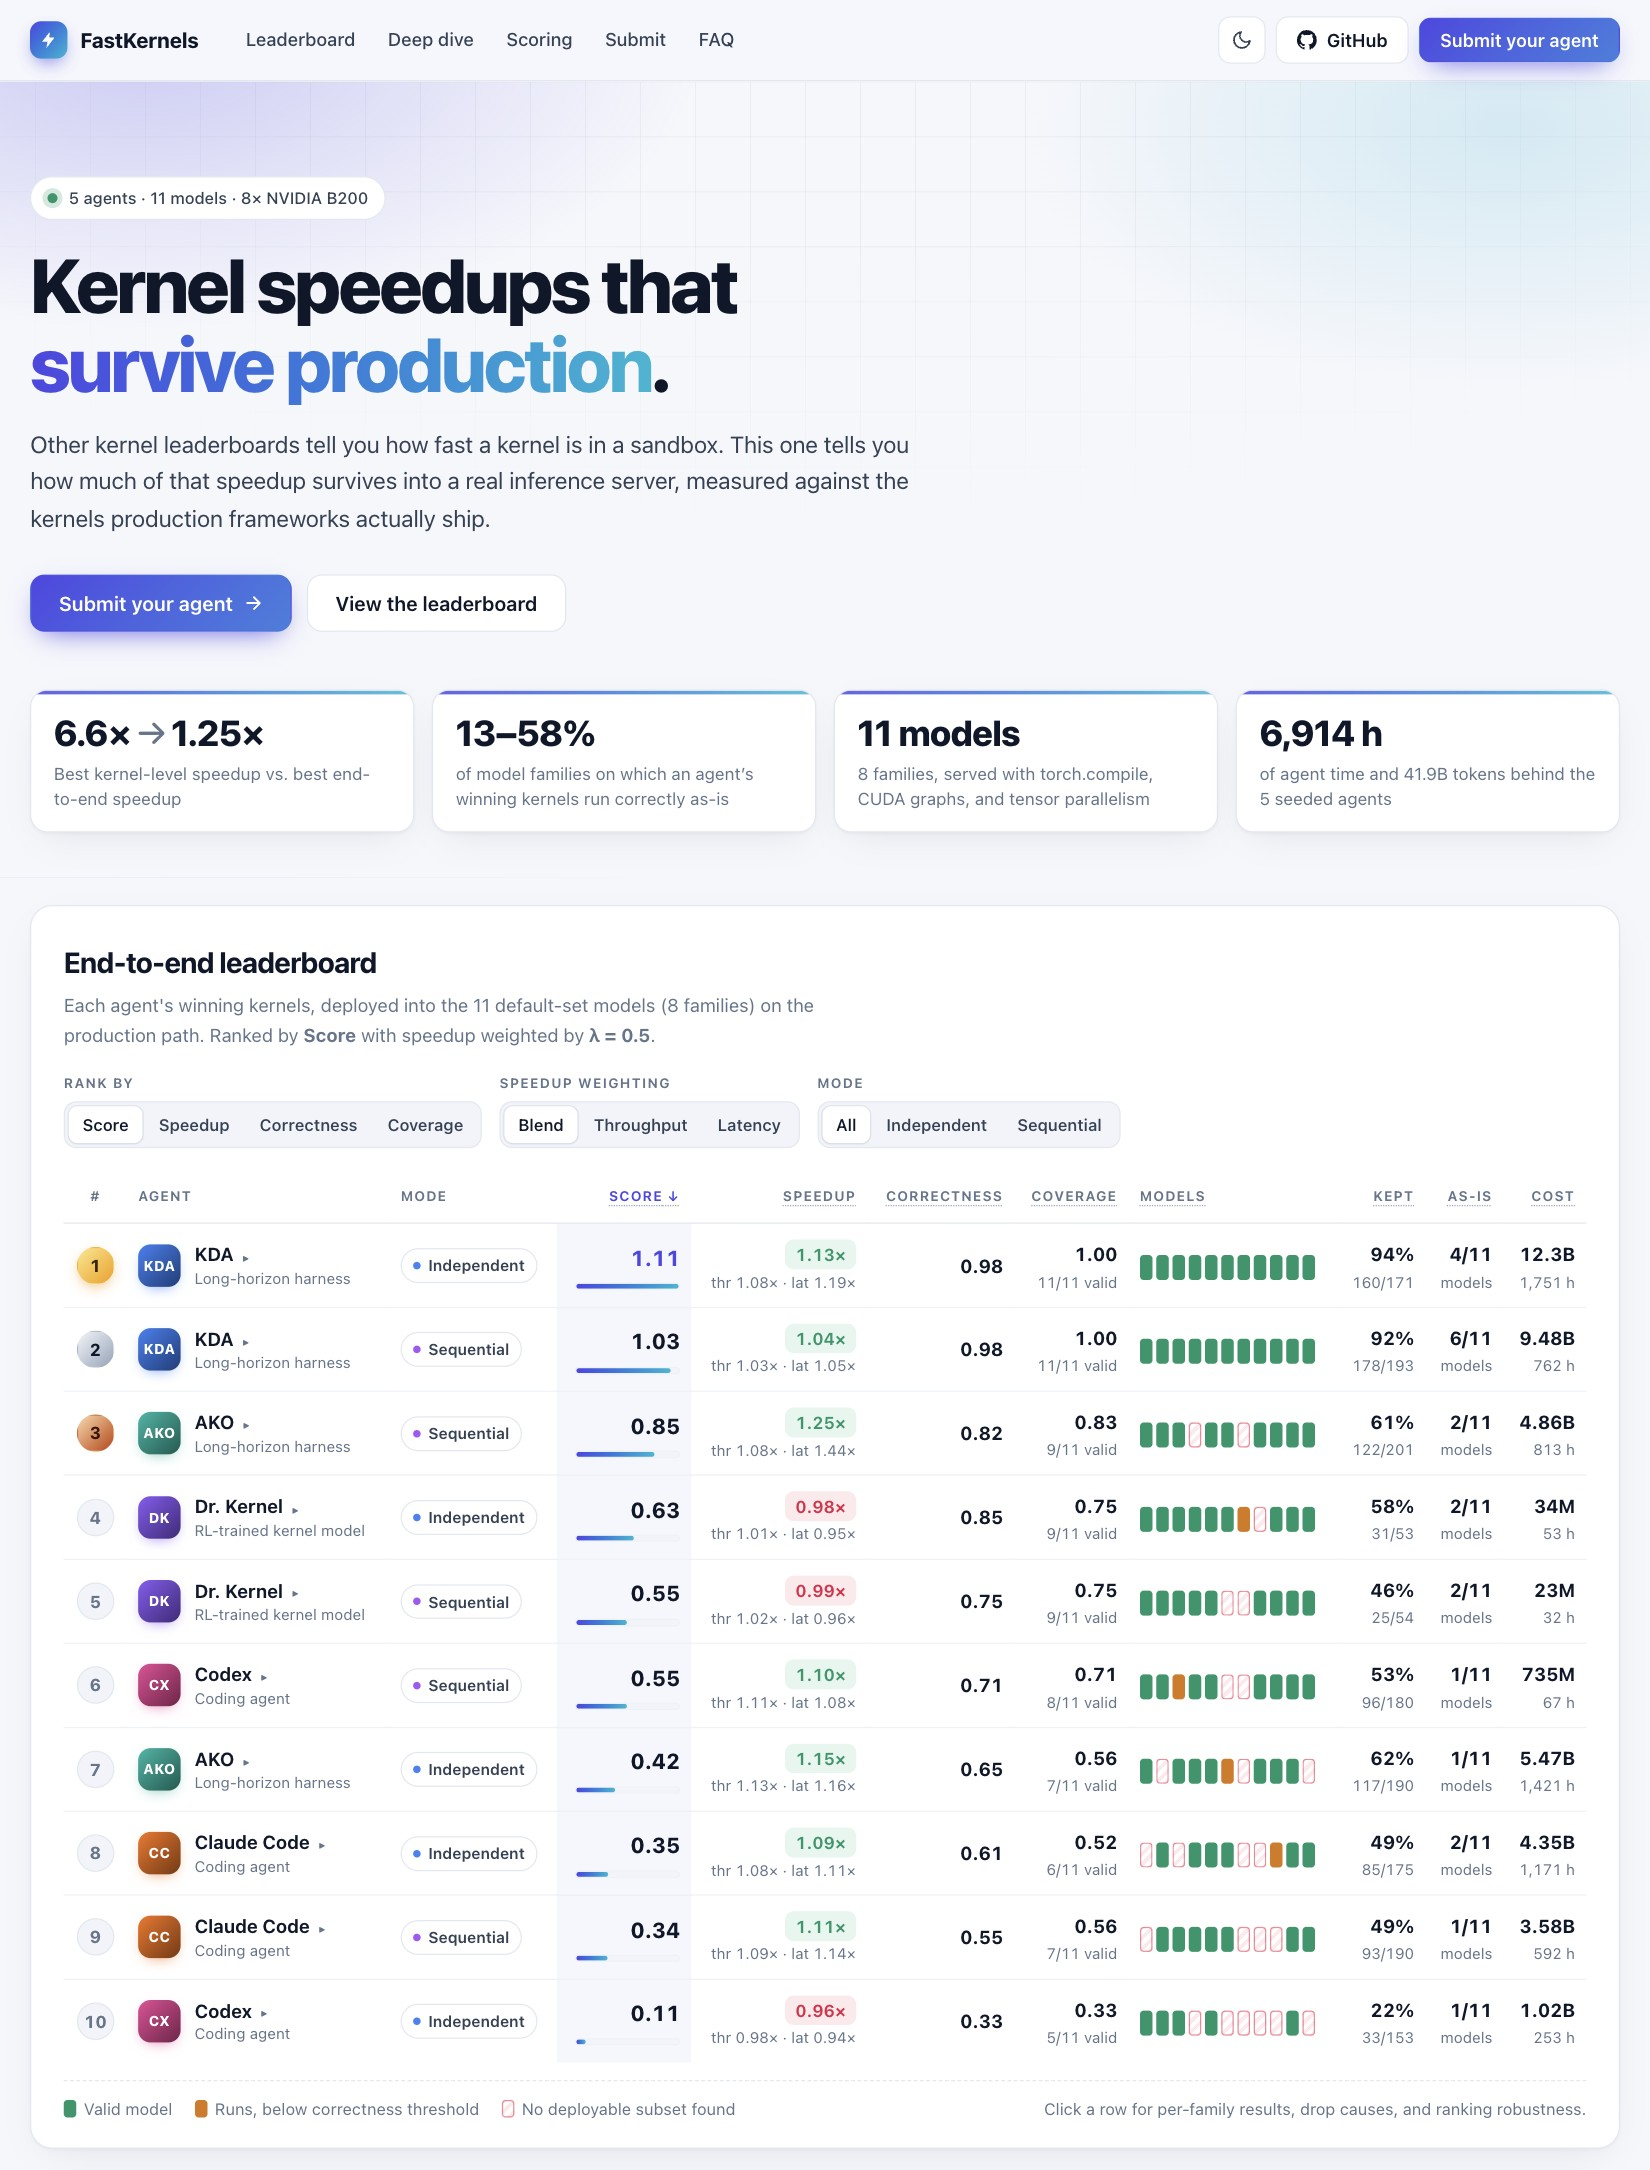
\includegraphics[width=\linewidth]{figures/leaderboard_overview.jpg}
  \caption{\textbf{Leaderboard.}}
  \label{fig:lb-overview}
\end{figure}

\begin{figure}[tbp]
  \centering
  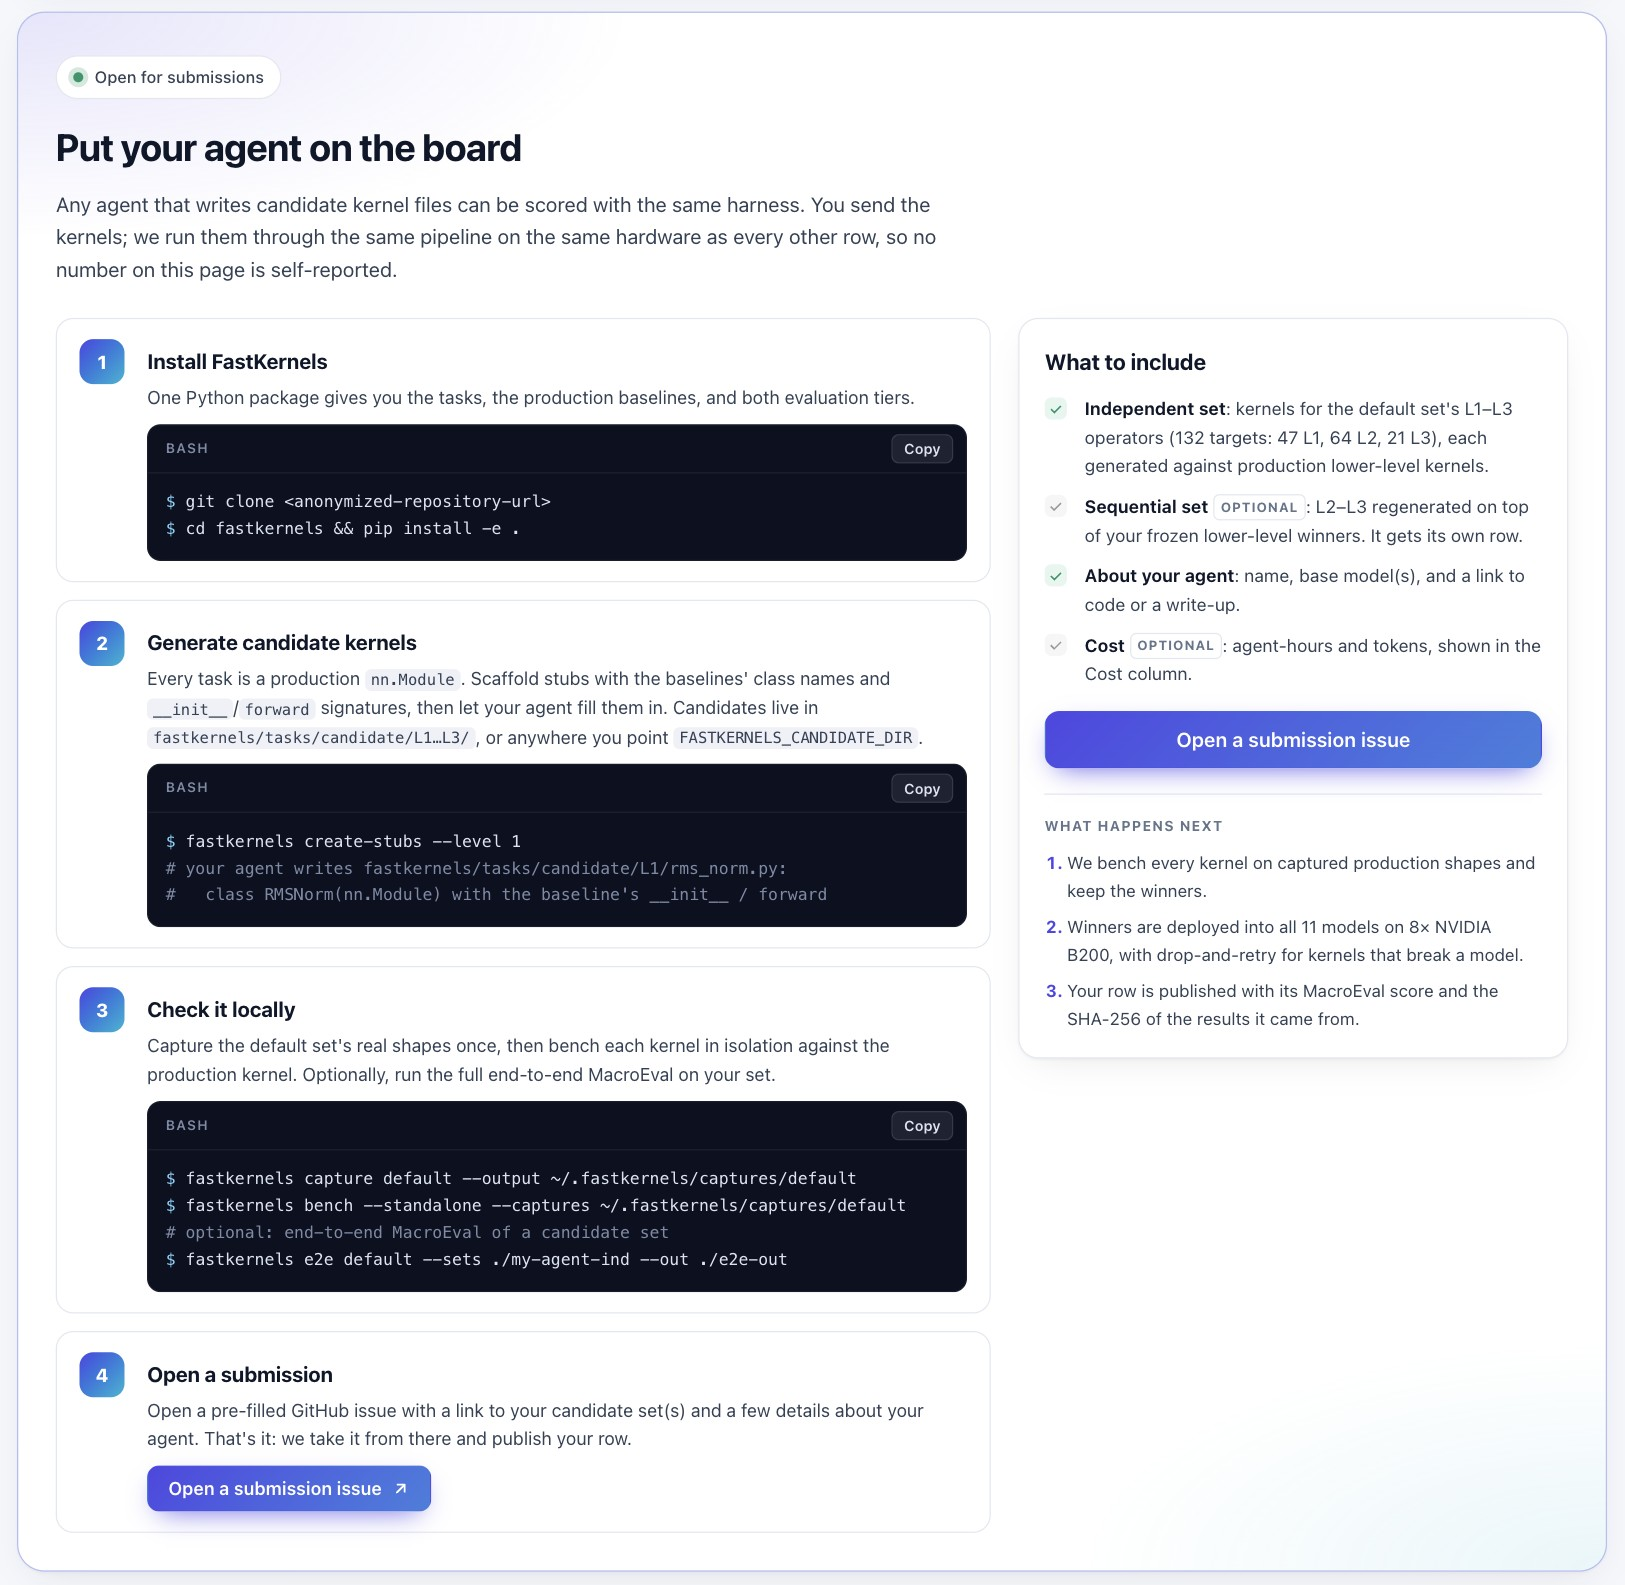
\includegraphics[width=\linewidth]{figures/leaderboard_submit.jpg}
  \ificlrfinal
  \caption{\textbf{Submission portal.}}
  \else
  \caption{\textbf{Submission portal.} Repository URL anonymized for review.}
  \fi
  \label{fig:lb-submit}
\end{figure}

\clearpage
\section{HuggingFace Transformers Coverage}
\label{app:hf_coverage}

We measure coverage empirically, by implementing every architecture in HuggingFace Transformers (commit \texttt{89b6b17}) on \fastkernels{}.
For each architecture, an agent implemented the model on top of the \fastkernels{} repository using only its existing operators: minimal patches were allowed, but no new operators or primitives.
To check correctness, we ran a few forward passes on a fixed batch whose input sizes exercise the model's relevant computation (e.g., for models with windowed attention, a sequence longer than the window): one step for non-autoregressive, embedding, and prefill-only models, and three steps (one prefill, two decodes) for autoregressive models.
We then compared the output of the \fastkernels{} implementation with that of native HF and consider the architecture supported if the implementation runs without errors and the relative L2 difference is within a \texttt{dtype}-dependent threshold: 0.01\% (FP32), 0.5\% (FP16), 2\% (BF16), 5\% (FP8), and 10--20\% (FP4); mixed-precision models use the threshold of their lowest-precision format.
Architectures without a public checkpoint use the constructor defaults of their HF configuration with random weights.

% Generated by figures/make_hf_coverage_table.py. Do not edit by hand.
Table~\ref{tab:hf-coverage} lists 488 architectures: 468 are within their threshold, 17 run but exceed it (marked $^\dagger$), and 4 (marked $^{*}$) are flagged by the HF audit only because the HF implementation differs from the version in the reference library \fastkernels{} pins (vLLM for \nolinkurl{kimi_linear}; FLA's RWKV-7 for \nolinkurl{rwkv}; the SAM~3 release for \nolinkurl{sam3_video}; timm for \nolinkurl{timm_wrapper}); we count these as supported because \fastkernels{} supports a valid version of each.
The remaining architectures fall in three groups.
\emph{Requiring new operations} (5): \nolinkurl{autoformer}, \nolinkurl{informer}, \nolinkurl{rag}, \nolinkurl{time_series_transformer}, \nolinkurl{xlstm}.
\emph{HF reference issues} (6), where the native HF implementation itself fails, so no reference output exists: \nolinkurl{deepseek_v4}, \nolinkurl{gemma4_assistant}, \nolinkurl{granite4_vision}, \nolinkurl{minicpmv4_7}, \nolinkurl{nllb_moe}, \nolinkurl{sam_hq}.
\emph{Excluded} (5): generic wrappers that compose other architectures and have no modeling code of their own: \nolinkurl{encoder_decoder}, \nolinkurl{speech_encoder_decoder}, \nolinkurl{timm_backbone}, \nolinkurl{vision_encoder_decoder}, \nolinkurl{vision_text_dual_encoder}.
Coverage is therefore \textbf{94.6\% (472/499)}: excluding the wrappers, the architectures above their threshold (unless marked $^{*}$), those that require new operations, and those without a working HF reference count as unsupported.


% Generated by figures/make_hf_coverage_table.py. Do not edit by hand.
\begingroup\scriptsize\setlength{\tabcolsep}{2pt}\setlength{\LTleft}{0pt}\setlength{\LTright}{0pt}
\begin{longtable}{@{}>{\raggedright\arraybackslash}p{.28\linewidth}>{\raggedright\arraybackslash}p{.45\linewidth}>{\raggedright\arraybackslash}p{.1\linewidth}>{\raggedleft\arraybackslash}p{.13\linewidth}@{}}
\caption{\textbf{HuggingFace Transformers coverage audit} (commit \texttt{89b6b17}): every architecture implemented on \fastkernels{} and the relative L2 difference (\%) of its output from native HF. $^\dagger$: above the threshold for its \texttt{dtype}. $^{*}$: flagged only because HF differs from the version \fastkernels{} pins; counted as supported.}\label{tab:hf-coverage}\\
\toprule
Architecture & HF model & \texttt{dtype} & Rel.\ L2 (\%) \\
\midrule
\endfirsthead
\multicolumn{4}{@{}l}{\tablename~\thetable\ (continued)}\\[2pt]
\toprule
Architecture & HF model & \texttt{dtype} & Rel.\ L2 (\%) \\
\midrule
\endhead
\bottomrule
\endfoot
\nolinkurl{afmoe} & \nolinkurl{arcee-ai/Trinity-Mini} & bf16 & 1.36 \\
\nolinkurl{aimv2} & \nolinkurl{apple/aimv2-large-patch14-224-lit} & bf16 & 0 \\
\nolinkurl{albert} & \nolinkurl{albert/albert-base-v2} & bf16 & 0.871 \\
\nolinkurl{align} & \nolinkurl{kakaobrain/align-base} & bf16 & 0 \\
\nolinkurl{altclip} & \nolinkurl{BAAI/AltCLIP} & bf16 & 0 \\
\nolinkurl{apertus} & \nolinkurl{swiss-ai/Apertus-8B-Instruct-2509} & bf16 & 0 \\
\nolinkurl{arcee} & \nolinkurl{arcee-ai/AFM-4.5B} & bf16 & 0.832 \\
\nolinkurl{aria} & \nolinkurl{Rhymes-AI/Aria} & bf16 & 0.518 \\
\nolinkurl{audio_spectrogram_transformer} & Constructor defaults & bf16 & 0 \\
\nolinkurl{audioflamingo3} & \nolinkurl{nvidia/audio-flamingo-3-hf} & bf16 & 0.639 \\
\nolinkurl{axk1} & \nolinkurl{skt/A.X-K1} & bf16 & 0.395 \\
\nolinkurl{axk2} & Constructor defaults & bf16 & 0.171 \\
\nolinkurl{aya_vision} & \nolinkurl{unsloth/aya-vision-8b} & bf16 & 0 \\
\nolinkurl{bamba} & \nolinkurl{ibm-ai-platform/Bamba-9B-v2} & bf16 & 0 \\
\nolinkurl{bark} & \nolinkurl{suno/bark} & bf16 & 0.913 \\
\nolinkurl{bart} & \nolinkurl{facebook/bart-large-cnn} & bf16 & 0 \\
\nolinkurl{beit} & Constructor defaults & bf16 & 0 \\
\nolinkurl{bert} & \nolinkurl{google-bert/bert-base-uncased} & bf16 & 0 \\
\nolinkurl{bert_generation} & \nolinkurl{google/bert_for_seq_generation_L-24_bbc_encoder} & bf16 & 0 \\
\nolinkurl{big_bird} & \nolinkurl{google/bigbird-roberta-base} & bf16 & 0 \\
\nolinkurl{bigbird_pegasus} & \nolinkurl{google/bigbird-pegasus-large-arxiv} & bf16 & 0 \\
\nolinkurl{biogpt} & \nolinkurl{microsoft/biogpt} & bf16 & 0 \\
\nolinkurl{bit} & Constructor defaults & bf16 & 0 \\
\nolinkurl{bitnet} & \nolinkurl{microsoft/bitnet-b1.58-2B-4T} & bf16 & 0 \\
\nolinkurl{blenderbot} & \nolinkurl{facebook/blenderbot-400M-distill} & bf16 & 0 \\
\nolinkurl{blenderbot_small} & \nolinkurl{facebook/blenderbot_small-90M} & bf16 & 0 \\
\nolinkurl{blip} & \nolinkurl{Salesforce/blip-image-captioning-base} & bf16 & 0 \\
\nolinkurl{blip_2} & \nolinkurl{Salesforce/blip2-opt-2.7b} & bf16 & 0 \\
\nolinkurl{blip_text} & Constructor defaults & bf16 & 0 \\
\nolinkurl{bloom} & \nolinkurl{bigscience/bloom} & bf16 & 0 \\
\nolinkurl{blt} & \nolinkurl{itazap/blt-1b-hf} & bf16 & 0 \\
\nolinkurl{bridgetower} & \nolinkurl{BridgeTower/bridgetower-base} & bf16 & 0 \\
\nolinkurl{bros} & \nolinkurl{jinho8345/bros-base-uncased} & bf16 & 0 \\
\nolinkurl{camembert} & \nolinkurl{almanach/camembert-base} & bf16 & 0 \\
\nolinkurl{canary} & \nolinkurl{nvidia/canary-1b-v2} & bf16 & 0 \\
\nolinkurl{canine} & Constructor defaults & fp32 & $1.95\!\times\!10^{-4}$ \\
\nolinkurl{chameleon} & \nolinkurl{nopperl/chameleon-7b-hf} & bf16 & 0.465 \\
\nolinkurl{chinese_clip} & \nolinkurl{OFA-Sys/chinese-clip-vit-base-patch16} & bf16 & 0 \\
\nolinkurl{chmv2} & Constructor defaults & bf16 & $6.32\!\times\!10^{-6}$ \\
\nolinkurl{clap} & \nolinkurl{laion/clap-htsat-unfused} & bf16 & 0 \\
\nolinkurl{clip} & \nolinkurl{openai/clip-vit-base-patch32} & bf16 & 0 \\
\nolinkurl{clipseg} & \nolinkurl{CIDAS/clipseg-rd64-refined} & bf16 & 1.35 \\
\nolinkurl{clvp} & \nolinkurl{susnato/clvp_dev} & fp32 & 0 \\
\nolinkurl{codegen} & \nolinkurl{Salesforce/codegen-350M-mono} & fp16 & 0 \\
\nolinkurl{cohere} & Constructor defaults & bf16 & 0 \\
\nolinkurl{cohere2} & Constructor defaults & bf16 & 0 \\
\nolinkurl{cohere2_moe} & \nolinkurl{CohereLabs/command-a-plus-05-2026} & bf16 & 0.528 \\
\nolinkurl{cohere2_vision} & \nolinkurl{mlx-community/command-a-vision-07-2025-4bit} & bf16 & 0.638 \\
\nolinkurl{cohere_asr} & Constructor defaults & bf16 & 0 \\
\nolinkurl{cohere_compass} & \nolinkurl{CohereLabs/North-Micro-Vision-Instruct} & bf16 & 0.789 \\
\nolinkurl{colmodernvbert} & ModernVBERT/colmodernvbert-merged + ColModernVBertConfig wrapper & bf16 & 0 \\
\nolinkurl{colpali} & vidore/colpaligemma-3b-pt-448-base + ColPaliConfig wrapper & bf16 & 1.01 \\
\nolinkurl{colqwen2} & \nolinkurl{vidore/colqwen2-v1.0-hf} & bf16 & 0.829 \\
\nolinkurl{conditional_detr} & \nolinkurl{microsoft/conditional-detr-resnet-50} & bf16 & 0 \\
\nolinkurl{convbert} & \nolinkurl{YituTech/conv-bert-base} & bf16 & 0 \\
\nolinkurl{convnext} & Constructor defaults & bf16 & 0 \\
\nolinkurl{convnextv2} & Constructor defaults & bf16 & 0 \\
\nolinkurl{cosmos3_edge} & \nolinkurl{nvidia/Cosmos3-Edge} & bf16 & 0 \\
\nolinkurl{cosmos3_omni} & \nolinkurl{nvidia/Cosmos3-Nano} & bf16 & 1.2 \\
\nolinkurl{cpmant} & \nolinkurl{openbmb/cpm-ant-10b} & bf16 & 0 \\
\nolinkurl{csm} & Constructor defaults & bf16 & 0.00206 \\
\nolinkurl{ctrl} & \nolinkurl{Salesforce/ctrl} & bf16 & 0.366 \\
\nolinkurl{cvt} & Constructor defaults & bf16 & 0 \\
\nolinkurl{cwm} & Constructor defaults & bf16 & 0.884 \\
\nolinkurl{d_fine} & \nolinkurl{ustc-community/dfine-xlarge-coco} & bf16 & 0 \\
\nolinkurl{dab_detr} & \nolinkurl{IDEA-Research/dab-detr-resnet-50} & fp32 & 0 \\
\nolinkurl{dac} & \nolinkurl{descript/dac_16khz} & bf16 & 0 \\
\nolinkurl{data2vec_audio} & Constructor defaults & bf16 & 0 \\
\nolinkurl{data2vec_text} & \nolinkurl{facebook/data2vec-text-base} & bf16 & 0 \\
\nolinkurl{data2vec_vision} & Constructor defaults & bf16 & 0 \\
\nolinkurl{dbrx} & alpindale/dbrx-instruct (mirror) & bf16 & 0 \\
\nolinkurl{deberta} & \nolinkurl{microsoft/deberta-base} & fp32 & $1.64\!\times\!10^{-4}$ \\
\nolinkurl{deberta_v2} & \nolinkurl{microsoft/deberta-v2-xlarge} & bf16 & 0 \\
\nolinkurl{decision_transformer} & \nolinkurl{edbeeching/decision-transformer-gym-hopper-medium} & bf16 & 0 \\
\nolinkurl{deepseek_ocr2} & \nolinkurl{deepseek-community/DeepSeek-OCR-2} & bf16 & 1.77 \\
\nolinkurl{deepseek_v2} & \nolinkurl{deepseek-ai/DeepSeek-V2-Lite} & bf16 & 1 \\
\nolinkurl{deepseek_v3} & \nolinkurl{deepseek-ai/DeepSeek-V3} & fp8/bf16 & 0 \\
\nolinkurl{deepseek_v32} & Constructor defaults & bf16 & 1.64 \\
\nolinkurl{deepseek_vl} & \nolinkurl{deepseek-community/deepseek-vl-1.3b-chat} & fp16 & 0.0769 \\
\nolinkurl{deepseek_vl_hybrid} & \nolinkurl{deepseek-community/deepseek-vl-7b-chat} & fp16 & 0.0693 \\
\nolinkurl{deformable_detr} & \nolinkurl{SenseTime/deformable-detr} & bf16 & 0 \\
\nolinkurl{deimv2} & \nolinkurl{harshaljanjani/DEIMv2_HGNetv2_N_COCO_Transformers} & bf16 & 0 \\
\nolinkurl{deit} & Constructor defaults & bf16 & 0 \\
\nolinkurl{depth_anything} & \nolinkurl{LiheYoung/depth-anything-small-hf} & bf16 & 0.141 \\
\nolinkurl{depth_pro} & \nolinkurl{apple/DepthPro-hf} & fp16 & 0.121 \\
\nolinkurl{detr} & \nolinkurl{facebook/detr-resnet-50-panoptic} & bf16 & 0 \\
\nolinkurl{dia} & Constructor defaults & bf16 & 0.537 \\
\nolinkurl{diffllama} & \nolinkurl{kajuma/DiffLlama-0.3B-handcut} & bf16 & 0.746 \\
\nolinkurl{diffusion_gemma} & \nolinkurl{google/diffusiongemma-26B-A4B-it} & bf16 & 81$^\dagger$ \\
\nolinkurl{dinat} & Constructor defaults & bf16 & 0 \\
\nolinkurl{dinov2} & Constructor defaults & bf16 & 0 \\
\nolinkurl{dinov2_with_registers} & Constructor defaults & bf16 & 0 \\
\nolinkurl{dinov3_convnext} & Constructor defaults & bf16 & 0 \\
\nolinkurl{dinov3_vit} & Constructor defaults & bf16 & 0 \\
\nolinkurl{distilbert} & \nolinkurl{distilbert/distilbert-base-uncased} & bf16 & 0.855 \\
\nolinkurl{doge} & Constructor defaults & bf16 & 0 \\
\nolinkurl{donut_swin} & Constructor defaults & bf16 & 0 \\
\nolinkurl{dots1} & \nolinkurl{rednote-hilab/dots.llm1.base} & bf16 & 0.239 \\
\nolinkurl{dpr} & \nolinkurl{facebook/dpr-question_encoder-single-nq-base} & bf16 & 0.972 \\
\nolinkurl{dpt} & Constructor defaults & bf16 & 0 \\
\nolinkurl{edgetam} & \nolinkurl{yonigozlan/EdgeTAM-hf} & bf16 & 0 \\
\nolinkurl{edgetam_video} & \nolinkurl{yonigozlan/EdgeTAM-hf} & bf16 & 0 \\
\nolinkurl{efficientloftr} & \nolinkurl{zju-community/efficientloftr} & bf16 & 0.0292 \\
\nolinkurl{efficientnet} & Constructor defaults & bf16 & 0 \\
\nolinkurl{electra} & \nolinkurl{google/electra-small-generator} & bf16 & 0.885 \\
\nolinkurl{emu3} & \nolinkurl{BAAI/Emu3-Chat-hf} & bf16 & 0 \\
\nolinkurl{encodec} & \nolinkurl{facebook/encodec_24khz} & bf16 & 0.0579 \\
\nolinkurl{eomt} & \nolinkurl{tue-mps/coco_panoptic_eomt_large_640} & bf16 & 0 \\
\nolinkurl{eomt_dinov3} & Constructor defaults & bf16 & 0 \\
\nolinkurl{ernie} & \nolinkurl{nghuyong/ernie-1.0-base-zh} & bf16 & 0 \\
\nolinkurl{ernie4_5} & \nolinkurl{baidu/ERNIE-4.5-0.3B-PT} & bf16 & 0 \\
\nolinkurl{ernie4_5_moe} & \nolinkurl{baidu/ERNIE-4.5-21B-A3B-PT} & bf16 & 0.542 \\
\nolinkurl{ernie4_5_vl_moe} & \nolinkurl{baidu/ERNIE-4.5-VL-28B-A3B-PT} & bf16 & 0.42 \\
\nolinkurl{esm} & \nolinkurl{facebook/esm-1b} & bf16 & 1.73 \\
\nolinkurl{esmc} & \nolinkurl{biohub/ESMC-6B-hf} & bf16 & 0 \\
\nolinkurl{esmfold} & \nolinkurl{facebook/esmfold_v1} & bf16 & $4.80\!\times\!10^{-6}$ \\
\nolinkurl{esmfold2} & \nolinkurl{biohub/ESMFold2-hf} & fp32 & $2.37\!\times\!10^{-5}$ \\
\nolinkurl{eurobert} & \nolinkurl{EuroBERT/EuroBERT-210m} & bf16 & 0 \\
\nolinkurl{evolla} & \nolinkurl{westlake-repl/Evolla-10B-DPO-hf} & bf16 & 0 \\
\nolinkurl{exaone4} & \nolinkurl{LGAI-EXAONE/EXAONE-4.0-32B} & bf16 & 0 \\
\nolinkurl{exaone4_5} & \nolinkurl{LGAI-EXAONE/EXAONE-4.5-33B} & bf16 & 1.27 \\
\nolinkurl{exaone_moe} & \nolinkurl{LGAI-EXAONE/K-EXAONE-236B-A23B} & bf16 & 1.65 \\
\nolinkurl{falcon} & \nolinkurl{tiiuae/falcon-7b-instruct} & bf16 & 1.45 \\
\nolinkurl{falcon_h1} & \nolinkurl{tiiuae/Falcon-H1-7B-Instruct} & bf16 & 1.25 \\
\nolinkurl{falcon_mamba} & \nolinkurl{tiiuae/falcon-mamba-7b-instruct} & bf16 & 0 \\
\nolinkurl{fast_vlm} & \nolinkurl{KamilaMila/FastVLM-0.5B} & bf16 & 0.69 \\
\nolinkurl{fastspeech2_conformer} & \nolinkurl{espnet/fastspeech2_conformer_with_hifigan} & fp32 & $1.91\!\times\!10^{-4}$ \\
\nolinkurl{flaubert} & \nolinkurl{flaubert/flaubert_base_uncased} & bf16 & 1.09 \\
\nolinkurl{flava} & \nolinkurl{facebook/flava-full} & bf16 & 0 \\
\nolinkurl{flex_olmo} & \nolinkurl{allenai/FlexOlmo-7x7B-1T} & bf16 & 0.86 \\
\nolinkurl{florence2} & \nolinkurl{florence-community/Florence-2-large} & fp16 & 0 \\
\nolinkurl{fnet} & \nolinkurl{google/fnet-base} & fp32 & $1.70\!\times\!10^{-4}$ \\
\nolinkurl{focalnet} & Constructor defaults & bf16 & 0 \\
\nolinkurl{fsmt} & \nolinkurl{facebook/wmt19-ru-en} & bf16 & 0 \\
\nolinkurl{fun_asr_nano} & \nolinkurl{FunAudioLLM/Fun-ASR-Nano-2512-hf} & bf16 & 0 \\
\nolinkurl{funnel} & \nolinkurl{funnel-transformer/small} & bf16 & 0 \\
\nolinkurl{fuyu} & \nolinkurl{adept/fuyu-8b} & bf16 & 0 \\
\nolinkurl{gemma} & Constructor defaults & bf16 & 0.451 \\
\nolinkurl{gemma2} & Constructor defaults & bf16 & 0.389 \\
\nolinkurl{gemma3} & Pinned Gemma3 4B recipe & bf16 & 0 \\
\nolinkurl{gemma3n} & Constructor defaults & bf16 & 0 \\
\nolinkurl{gemma4} & \nolinkurl{google/gemma-4-e2b-it} & bf16 & 0 \\
\nolinkurl{gemma4_unified} & \nolinkurl{google/gemma-4-12B-it} & bf16 & 5.88$^\dagger$ \\
\nolinkurl{gemma4_unified_assistant} & \nolinkurl{google/gemma-4-e2b-it-assistant} & bf16 & 0 \\
\nolinkurl{git} & \nolinkurl{microsoft/git-base-coco} & bf16 & 0 \\
\nolinkurl{glm} & \nolinkurl{THUDM/glm-4-9b-chat} & bf16 & 0.905 \\
\nolinkurl{glm4} & Constructor defaults & bf16 & 0.761 \\
\nolinkurl{glm46v} & \nolinkurl{zai-org/GLM-4.1V-9B-Thinking} & bf16 & 0 \\
\nolinkurl{glm4_moe} & \nolinkurl{zai-org/GLM-4.5} & bf16 & 0.212 \\
\nolinkurl{glm4_moe_lite} & \nolinkurl{zai-org/GLM-4.7-Flash} & bf16 & 0.99 \\
\nolinkurl{glm4v} & \nolinkurl{zai-org/GLM-4.1V-9B-Thinking} & bf16 & 0 \\
\nolinkurl{glm4v_moe} & \nolinkurl{zai-org/GLM-4.5V} & bf16 & 0.143 \\
\nolinkurl{glm5_next} & \nolinkurl{zai-org/GLM-5.3-Flash} & fp8/bf16 & 19.5$^\dagger$ \\
\nolinkurl{glm_image} & \nolinkurl{zai-org/GLM-Image} & bf16 & 0 \\
\nolinkurl{glm_moe_dsa} & \nolinkurl{zai-org/GLM-5} & bf16 & 1.92 \\
\nolinkurl{glm_ocr} & \nolinkurl{zai-org/GLM-OCR} & bf16 & 0 \\
\nolinkurl{glmasr} & \nolinkurl{zai-org/GLM-ASR-Nano-2512} & bf16 & 0 \\
\nolinkurl{glpn} & \nolinkurl{vinvino02/glpn-kitti} & bf16 & 0.062 \\
\nolinkurl{got_ocr2} & \nolinkurl{stepfun-ai/GOT-OCR-2.0-hf} & bf16 & 0 \\
\nolinkurl{gpt2} & \nolinkurl{openai-community/gpt2} & bf16 & 0 \\
\nolinkurl{gpt_bigcode} & \nolinkurl{bigcode/gpt_bigcode-santacoder} & bf16 & 0 \\
\nolinkurl{gpt_neo} & \nolinkurl{EleutherAI/gpt-neo-1.3B} & bf16 & 0 \\
\nolinkurl{gpt_neox} & \nolinkurl{EleutherAI/gpt-neox-20b} & fp16 & 0.0522 \\
\nolinkurl{gpt_neox_japanese} & \nolinkurl{abeja/gpt-neox-japanese-2.7b} & bf16 & 0.687 \\
\nolinkurl{gpt_oss} & \nolinkurl{openai/gpt-oss-20b} & mxfp4/bf16 & 0 \\
\nolinkurl{gptj} & \nolinkurl{EleutherAI/gpt-j-6B} & bf16 & 0 \\
\nolinkurl{granite} & \nolinkurl{ibm-granite/granite-3.0-8b-base} & bf16 & 0.275 \\
\nolinkurl{granite_speech} & \nolinkurl{ibm-granite/granite-speech-3.3-2b} & bf16 & 0 \\
\nolinkurl{granite_speech5} & \nolinkurl{ibm-granite/granite-speech-5.0-470m-turboctc} & bf16 & 0 \\
\nolinkurl{granite_speech_plus} & \nolinkurl{ibm-granite/granite-speech-4.1-2b-plus} & bf16 & 0 \\
\nolinkurl{granite_swa} & \nolinkurl{ibm-granite/granite-swash-2b} & bf16 & 0 \\
\nolinkurl{granitemoe} & \nolinkurl{ibm/PowerMoE-3b} & bf16 & 1.69 \\
\nolinkurl{granitemoe_swa} & \nolinkurl{ibm-granite/granite-swash-3b-a600m} & bf16 & 9.34$^\dagger$ \\
\nolinkurl{granitemoehybrid} & \nolinkurl{ibm-granite/granite-4.0-h-tiny} & bf16 & 0 \\
\nolinkurl{granitemoeshared} & \nolinkurl{ibm-research/moe-7b-1b-active-shared-experts} & bf16 & 0 \\
\nolinkurl{grounding_dino} & \nolinkurl{IDEA-Research/grounding-dino-tiny} & fp32 & $6.4\!\times\!10^{-5}$ \\
\nolinkurl{groupvit} & \nolinkurl{nvidia/groupvit-gcc-yfcc} & bf16 & 0 \\
\nolinkurl{helium} & \nolinkurl{kyutai/helium-1-preview} & bf16 & 0 \\
\nolinkurl{hgnet_v2} & Constructor defaults & bf16 & 0 \\
\nolinkurl{hiera} & Constructor defaults & bf16 & 0 \\
\nolinkurl{higgs_audio_v2} & \nolinkurl{eustlb/higgs-audio-v2-generation-3B-base} & bf16 & 0 \\
\nolinkurl{higgs_audio_v2_tokenizer} & \nolinkurl{eustlb/higgs-audio-v2-tokenizer} & bf16 & 0 \\
\nolinkurl{hrm_text} & \nolinkurl{sapientinc/HRM-Text-1B} & bf16 & 0 \\
\nolinkurl{hubert} & \nolinkurl{facebook/hubert-large-ls960-ft} & bf16 & 0 \\
\nolinkurl{hunyuan_v1_dense} & \nolinkurl{tencent/Hunyuan-0.5B-Pretrain} & bf16 & 0 \\
\nolinkurl{hunyuan_v1_moe} & \nolinkurl{tencent/Hunyuan-A13B-Instruct} & bf16 & 0 \\
\nolinkurl{hunyuan_vl} & \nolinkurl{tencent/HunyuanOCR} & bf16 & 0.724 \\
\nolinkurl{hy_v3} & \nolinkurl{tencent/Hy3-preview} & bf16 & 0.712 \\
\nolinkurl{hy_v4} & \nolinkurl{tencent/Hy4-preview} & bf16 & 2.55$^\dagger$ \\
\nolinkurl{hyperclovax} & \nolinkurl{naver-hyperclovax/HyperCLOVAX-SEED-Think-14B} & bf16 & 0 \\
\nolinkurl{hyperclovax_vision_v2} & \nolinkurl{naver-hyperclovax/HyperCLOVAX-SEED-Think-32B} & bf16 & 0.78 \\
\nolinkurl{ibert} & \nolinkurl{kssteven/ibert-roberta-base} & bf16 & 1.33 \\
\nolinkurl{idefics} & \nolinkurl{HuggingFaceM4/idefics-9b} & bf16 & 0.651 \\
\nolinkurl{idefics2} & \nolinkurl{HuggingFaceM4/idefics2-8b-base} & bf16 & 0.749 \\
\nolinkurl{idefics3} & \nolinkurl{HuggingFaceM4/Idefics3-8B-Llama3} & bf16 & 1.12 \\
\nolinkurl{ijepa} & Constructor defaults & bf16 & 0 \\
\nolinkurl{imagegpt} & \nolinkurl{openai/imagegpt-small} & bf16 & 0 \\
\nolinkurl{inkling} & \nolinkurl{thinkingmachines/Inkling} & bf16 & 4.15$^\dagger$ \\
\nolinkurl{instructblip} & \nolinkurl{Salesforce/instructblip-vicuna-7b} & bf16 & 0.539 \\
\nolinkurl{instructblipvideo} & \nolinkurl{Salesforce/instructblip-vicuna-7b} & bf16 & 0.483 \\
\nolinkurl{internvl} & \nolinkurl{OpenGVLab/InternVL3-1B-hf} & bf16 & 0 \\
\nolinkurl{jais2} & Constructor defaults & bf16 & 0 \\
\nolinkurl{jamba} & \nolinkurl{ai21labs/Jamba-v0.1} & bf16 & 1.02 \\
\nolinkurl{janus} & \nolinkurl{deepseek-community/Janus-Pro-1B} & bf16 & 0 \\
\nolinkurl{jetmoe} & \nolinkurl{jetmoe/jetmoe-8b} & bf16 & 0.341 \\
\nolinkurl{jina_embeddings_v3} & \nolinkurl{jinaai/jina-embeddings-v3-hf} & bf16 & 1.5 \\
\nolinkurl{kimi_k25} & \nolinkurl{moonshotai/Kimi-K2.6} & int4/bf16 & 7.61 \\
\nolinkurl{kimi_linear}$^{*}$ & \nolinkurl{moonshotai/Kimi-Linear-48B-A3B-Instruct} & bf16 & 16.9$^\dagger$ \\
\nolinkurl{kosmos2} & \nolinkurl{microsoft/kosmos-2-patch14-224} & bf16 & 0 \\
\nolinkurl{kosmos2_5} & \nolinkurl{microsoft/kosmos-2.5} & bf16 & 0 \\
\nolinkurl{kyutai_speech_to_text} & \nolinkurl{kyutai/stt-2.6b-en-trfs} & bf16 & 0 \\
\nolinkurl{laguna} & \nolinkurl{poolside/laguna-XS.2} & bf16 & 0 \\
\nolinkurl{lasr} & Constructor defaults & bf16 & 0.727 \\
\nolinkurl{layoutlm} & \nolinkurl{microsoft/layoutlm-base-uncased} & bf16 & 0 \\
\nolinkurl{layoutlmv2} & \nolinkurl{microsoft/layoutlmv2-base-uncased} & bf16 & 0 \\
\nolinkurl{layoutlmv3} & \nolinkurl{microsoft/layoutlmv3-base} & bf16 & 0 \\
\nolinkurl{led} & \nolinkurl{allenai/led-large-16384-arxiv} & bf16 & 0 \\
\nolinkurl{levit} & Constructor defaults & bf16 & 0 \\
\nolinkurl{lfm2} & \nolinkurl{LiquidAI/LFM2-1.2B} & bf16 & 1.83 \\
\nolinkurl{lfm2_moe} & \nolinkurl{LiquidAI/LFM2-8B-A1B} & bf16 & 1.45 \\
\nolinkurl{lfm2_vl} & \nolinkurl{LiquidAI/LFM2-VL-1.6B} & bf16 & 0.787 \\
\nolinkurl{lightglue} & \nolinkurl{ETH-CVG/lightglue_superpoint} & bf16 & 0 \\
\nolinkurl{lighton_ocr} & \nolinkurl{lightonai/LightOnOCR-1B-1025} & bf16 & 0 \\
\nolinkurl{lilt} & \nolinkurl{SCUT-DLVCLab/lilt-roberta-en-base} & bf16 & 0 \\
\nolinkurl{llama} & Constructor defaults & bf16 & 0.746 \\
\nolinkurl{llama4} & Constructor defaults & bf16 & 0 \\
\nolinkurl{llava} & \nolinkurl{llava-hf/llava-1.5-7b-hf} & fp16 & 0.0932 \\
\nolinkurl{llava_next} & \nolinkurl{llava-hf/llava-v1.6-mistral-7b-hf} & fp16 & 0.0961 \\
\nolinkurl{llava_next_video} & \nolinkurl{llava-hf/LLaVA-NeXT-Video-7B-hf} & bf16 & 1.34 \\
\nolinkurl{llava_onevision} & \nolinkurl{llava-hf/llava-onevision-qwen2-7b-ov-hf} & fp16 & 0.0756 \\
\nolinkurl{longcat_flash} & \nolinkurl{meituan-longcat/LongCat-Flash-Chat} & bf16 & 0.725 \\
\nolinkurl{longformer} & \nolinkurl{allenai/longformer-base-4096} & bf16 & 0 \\
\nolinkurl{longt5} & \nolinkurl{Stancld/longt5-tglobal-large-16384-pubmed-3k_steps} & bf16 & 0 \\
\nolinkurl{luke} & \nolinkurl{studio-ousia/luke-base} & bf16 & 0 \\
\nolinkurl{lw_detr} & \nolinkurl{AnnaZhang/lwdetr_small_60e_coco} & bf16 & 0 \\
\nolinkurl{lxmert} & \nolinkurl{unc-nlp/lxmert-base-uncased} & bf16 & 0 \\
\nolinkurl{m2m_100} & \nolinkurl{facebook/m2m100_418M} & bf16 & 0 \\
\nolinkurl{mamba} & \nolinkurl{state-spaces/mamba-130m-hf} & bf16 & 0 \\
\nolinkurl{mamba2} & \nolinkurl{mistralai/Mamba-Codestral-7B-v0.1} & bf16 & 0 \\
\nolinkurl{marian} & \nolinkurl{Helsinki-NLP/opus-mt-en-de} & bf16 & 0 \\
\nolinkurl{markuplm} & \nolinkurl{microsoft/markuplm-base} & fp16 & 0 \\
\nolinkurl{mask2former} & \nolinkurl{facebook/mask2former-swin-small-coco-instance} & bf16 & 0 \\
\nolinkurl{maskformer} & \nolinkurl{facebook/maskformer-swin-base-ade} & fp32 & 0 \\
\nolinkurl{maskformer_swin} & Constructor defaults & fp32 & $2.82\!\times\!10^{-5}$ \\
\nolinkurl{mbart} & \nolinkurl{facebook/mbart-large-en-ro} & bf16 & 0 \\
\nolinkurl{megatron_bert} & Constructor defaults & bf16 & 0 \\
\nolinkurl{mellum} & \nolinkurl{JetBrains/Mellum2-12B-A2.5B-Base} & bf16 & 0.817 \\
\nolinkurl{metaclip_2} & \nolinkurl{facebook/metaclip-2-worldwide-huge-quickgelu} & bf16 & 0 \\
\nolinkurl{mgp_str} & \nolinkurl{alibaba-damo/mgp-str-base} & bf16 & 0.365 \\
\nolinkurl{mimi} & \nolinkurl{kyutai/mimi} & bf16 & 0 \\
\nolinkurl{mimo_v2_flash} & \nolinkurl{XiaomiMiMo/MiMo-V2-Flash} & fp8/bf16 & 12.2$^\dagger$ \\
\nolinkurl{minicpm3} & \nolinkurl{openbmb/MiniCPM3-4B} & bf16 & 0 \\
\nolinkurl{minicpmv4_6} & \nolinkurl{openbmb/MiniCPM-V-4_6} & bf16 & 1.27 \\
\nolinkurl{minimax} & \nolinkurl{MiniMaxAI/MiniMax-Text-01-hf} & bf16 & 0.255 \\
\nolinkurl{minimax_m2} & \nolinkurl{MiniMaxAI/MiniMax-M2} & fp8/bf16 & $8.69\!\times\!10^{-5}$ \\
\nolinkurl{minimax_m3_vl} & \nolinkurl{MiniMaxAI/MiniMax-M3} & bf16 & 3.4$^\dagger$ \\
\nolinkurl{ministral} & \nolinkurl{mistralai/Ministral-8B-Instruct-2410} & bf16 & 0.768 \\
\nolinkurl{ministral3} & \nolinkurl{mistralai/Ministral-3-8B-Base-2512} & bf16 & 0.649 \\
\nolinkurl{mistral} & \nolinkurl{mistralai/Mistral-7B-v0.1} & bf16 & 0.81 \\
\nolinkurl{mistral3} & \nolinkurl{mistralai/Mistral-Small-3.1-24B-Instruct-2503} & bf16 & 0 \\
\nolinkurl{mistral4} & \nolinkurl{mistralai/Mistral-Small-4-119B-2603} & fp8/bf16/fp32 & 0 \\
\nolinkurl{mixtral} & \nolinkurl{mistralai/Mixtral-8x7B-v0.1} & bf16 & 0 \\
\nolinkurl{mlcd} & \nolinkurl{DeepGlint-AI/mlcd-vit-bigG-patch14-448} & bf16 & 1.24 \\
\nolinkurl{mllama} & Constructor defaults & bf16 & 0 \\
\nolinkurl{mm_grounding_dino} & \nolinkurl{openmmlab-community/mm_grounding_dino_tiny_o365v1_goldg_v3det} & fp32 & $4.4\!\times\!10^{-5}$ \\
\nolinkurl{mobilebert} & \nolinkurl{google/mobilebert-uncased} & bf16 & 0 \\
\nolinkurl{mobilenet_v1} & Constructor defaults & bf16 & 0 \\
\nolinkurl{mobilenet_v2} & Constructor defaults & bf16 & 0 \\
\nolinkurl{mobilevit} & Constructor defaults & bf16 & 0 \\
\nolinkurl{mobilevitv2} & Constructor defaults & bf16 & 0.701 \\
\nolinkurl{modernbert} & \nolinkurl{answerdotai/ModernBERT-base} & bf16 & 0 \\
\nolinkurl{modernbert_decoder} & \nolinkurl{blab-jhu/test-32m-dec} & bf16 & 0 \\
\nolinkurl{modernvbert} & \nolinkurl{ModernVBERT/modernvbert} & bf16 & 1.3 \\
\nolinkurl{moonshine} & \nolinkurl{UsefulSensors/moonshine-tiny} & bf16 & 0 \\
\nolinkurl{moonshine_streaming} & \nolinkurl{UsefulSensors/moonshine-streaming-tiny} & bf16 & 0 \\
\nolinkurl{moshi} & \nolinkurl{kmhf/hf-moshiko} & bf16 & 0 \\
\nolinkurl{mpnet} & \nolinkurl{microsoft/mpnet-base} & bf16 & 0 \\
\nolinkurl{mpt} & Constructor defaults & bf16 & 0 \\
\nolinkurl{mra} & \nolinkurl{uw-madison/mra-base-512-4} & fp32 & $4.1\!\times\!10^{-5}$ \\
\nolinkurl{mt5} & \nolinkurl{google/mt5-small} & bf16 & 0 \\
\nolinkurl{muse_glimmer} & \nolinkurl{meta-models/Muse-Glimmer-30B} & bf16 & 12.2$^\dagger$ \\
\nolinkurl{muse_glimmer_assistant} & \nolinkurl{meta-models/Muse-Glimmer-30B-assistant} & bf16 & 0.413 \\
\nolinkurl{musicflamingo} & \nolinkurl{nvidia/music-flamingo-2601-hf} & bf16 & 0 \\
\nolinkurl{musicgen} & \nolinkurl{facebook/musicgen-small} & bf16 & 0 \\
\nolinkurl{musicgen_melody} & \nolinkurl{facebook/musicgen-melody} & bf16 & 0 \\
\nolinkurl{mvp} & \nolinkurl{RUCAIBox/mvp} & bf16 & 0 \\
\nolinkurl{nanochat} & Constructor defaults & bf16 & 0 \\
\nolinkurl{nemotron} & \nolinkurl{nvidia/Minitron-4B-Base} & bf16 & 0.843 \\
\nolinkurl{nemotron3_5_asr} & \nolinkurl{nvidia/nemotron-3.5-asr-streaming-0.6b} & bf16 & 0.0547 \\
\nolinkurl{nemotron3_diarization} & \nolinkurl{nvidia/Nemotron-3-Diarization} & bf16 & 0 \\
\nolinkurl{nemotron_asr_streaming} & \nolinkurl{nvidia/nemotron-speech-streaming-en-0.6b} & bf16 & 0.569 \\
\nolinkurl{nemotron_h} & \nolinkurl{nvidia/Nemotron-H-8B-Reasoning-128K} & bf16 & 1.53 \\
\nolinkurl{nemotron_h_omni} & \nolinkurl{nvidia/Nemotron-3-Nano-Omni-30B-A3B-Reasoning-BF16} & bf16 & 13.2$^\dagger$ \\
\nolinkurl{neomme} & \nolinkurl{Hcompany/NeoMME-260M} & bf16 & 0.118 \\
\nolinkurl{neucodec} & Constructor defaults & bf16 & 16.1$^\dagger$ \\
\nolinkurl{nomic_bert} & Constructor defaults & bf16 & 0 \\
\nolinkurl{nystromformer} & \nolinkurl{uw-madison/nystromformer-512} & bf16 & 0 \\
\nolinkurl{olmo} & \nolinkurl{allenai/OLMo-7B-hf} & bf16 & 0.711 \\
\nolinkurl{olmo2} & \nolinkurl{allenai/OLMo-2-0425-1B} & bf16 & 0 \\
\nolinkurl{olmo3} & \nolinkurl{allenai/Olmo-3-7B-Instruct} & bf16 & 0 \\
\nolinkurl{olmo_hybrid} & \nolinkurl{allenai/Olmo-Hybrid-7B} & bf16 & 0.639 \\
\nolinkurl{olmoe} & \nolinkurl{allenai/OLMoE-1B-7B-0924} & bf16 & 0.557 \\
\nolinkurl{omdet_turbo} & \nolinkurl{omlab/omdet-turbo-swin-tiny-hf} & bf16 & 0 \\
\nolinkurl{oneformer} & \nolinkurl{shi-labs/oneformer_ade20k_swin_tiny} & bf16 & 0.302 \\
\nolinkurl{openai} & \nolinkurl{openai-community/openai-gpt} & bf16 & 0 \\
\nolinkurl{openai_privacy_filter} & \nolinkurl{openai/privacy-filter} & bf16 & 1.3 \\
\nolinkurl{opt} & \nolinkurl{facebook/opt-350m} & fp16 & 0 \\
\nolinkurl{ovis2} & \nolinkurl{thisisiron/Ovis2-2B-hf} & bf16 & 0.702 \\
\nolinkurl{owlv2} & \nolinkurl{google/owlv2-base-patch16-ensemble} & bf16 & 0 \\
\nolinkurl{owlvit} & \nolinkurl{google/owlvit-base-patch32} & bf16 & 0 \\
\nolinkurl{paddleocr_vl} & \nolinkurl{PaddlePaddle/PaddleOCR-VL} & bf16 & 0 \\
\nolinkurl{paligemma} & Constructor defaults & bf16 & 0.0153 \\
\nolinkurl{parakeet} & \nolinkurl{nvidia/parakeet-ctc-1.1b} & bf16 & 0 \\
\nolinkurl{patchtsmixer} & \nolinkurl{ibm/patchtsmixer-etth1-pretrain} & bf16 & 0 \\
\nolinkurl{patchtst} & \nolinkurl{namctin/patchtst_etth1_pretrain} & bf16 & 0.132 \\
\nolinkurl{pe_audio} & \nolinkurl{facebook/pe-av-large} & bf16 & 0 \\
\nolinkurl{pe_audio_video} & \nolinkurl{facebook/pe-av-large} & bf16 & 0 \\
\nolinkurl{pe_video} & \nolinkurl{facebook/pe-av-large} & bf16 & 0 \\
\nolinkurl{pegasus} & \nolinkurl{google/pegasus-xsum} & bf16 & 0 \\
\nolinkurl{pegasus_x} & \nolinkurl{google/pegasus-x-large} & bf16 & 0 \\
\nolinkurl{perceiver} & Constructor defaults & bf16 & 0 \\
\nolinkurl{perception_lm} & \nolinkurl{facebook/Perception-LM-1B} & bf16 & 0 \\
\nolinkurl{persimmon} & \nolinkurl{adept/persimmon-8b-base} & bf16 & 0 \\
\nolinkurl{phi} & \nolinkurl{microsoft/phi-1} & bf16 & 0 \\
\nolinkurl{phi3} & \nolinkurl{microsoft/Phi-3-mini-4k-instruct} & bf16 & 0.929 \\
\nolinkurl{phi4_multimodal (speech)} & \nolinkurl{microsoft/Phi-4-multimodal-instruct} & bf16 & 0 \\
\nolinkurl{phimoe} & \nolinkurl{microsoft/Phi-3.5-MoE-instruct} & bf16 & 0 \\
\nolinkurl{pi0} & Constructor defaults & bf16 & 0.282 \\
\nolinkurl{pix2struct} & \nolinkurl{google/pix2struct-textcaps-base} & bf16 & 0 \\
\nolinkurl{pixio} & Constructor defaults & bf16 & 0 \\
\nolinkurl{pixtral} & \nolinkurl{mistral-labs/pixtral-12b} & bf16 & 0 \\
\nolinkurl{plbart} & \nolinkurl{uclanlp/plbart-base} & bf16 & 0 \\
\nolinkurl{poolformer} & Constructor defaults & bf16 & 0 \\
\nolinkurl{pop2piano} & \nolinkurl{sweetcocoa/pop2piano} & bf16 & 0 \\
\nolinkurl{pp_doclayout_v2} & \nolinkurl{PaddlePaddle/PP-DocLayoutV2_safetensors} & bf16 & 0 \\
\nolinkurl{pp_doclayout_v3} & \nolinkurl{PaddlePaddle/PP-DocLayoutV3_safetensors} & bf16 & 0 \\
\nolinkurl{pp_formulanet} & \nolinkurl{PaddlePaddle/PP-FormulaNet_plus-L_safetensors} & bf16 & 0 \\
\nolinkurl{pp_lcnet} & Constructor defaults & bf16 & 0 \\
\nolinkurl{pp_lcnet_v3} & Constructor defaults & bf16 & 0 \\
\nolinkurl{pp_lcnet_v4} & Constructor defaults & bf16 & 0 \\
\nolinkurl{pp_ocrv5_mobile_det} & \nolinkurl{PaddlePaddle/PP-OCRv5_mobile_det_safetensors} & bf16 & 0 \\
\nolinkurl{pp_ocrv5_mobile_rec} & \nolinkurl{PaddlePaddle/PP-OCRv5_mobile_rec_safetensors} & bf16 & 0 \\
\nolinkurl{pp_ocrv5_server_det} & \nolinkurl{PaddlePaddle/PP-OCRv5_server_det_safetensors} & bf16 & 0 \\
\nolinkurl{pp_ocrv5_server_rec} & \nolinkurl{PaddlePaddle/PP-OCRv5_server_rec_safetensors} & bf16 & 0 \\
\nolinkurl{pp_ocrv6_medium_det} & \nolinkurl{PaddlePaddle/PP-OCRv6_medium_det_safetensors} & bf16 & 0 \\
\nolinkurl{pp_ocrv6_small_det} & \nolinkurl{PaddlePaddle/PP-OCRv6_small_det_safetensors} & bf16 & 0 \\
\nolinkurl{pp_ocrv6_small_rec} & \nolinkurl{PaddlePaddle/PP-OCRv6_small_rec_safetensors} & bf16 & 0 \\
\nolinkurl{pp_ocrv6_tiny_rec} & \nolinkurl{PaddlePaddle/PP-OCRv6_tiny_rec_safetensors} & bf16 & 0 \\
\nolinkurl{prompt_depth_anything} & \nolinkurl{depth-anything/prompt-depth-anything-vits-hf} & bf16 & 0.0479 \\
\nolinkurl{prophetnet} & \nolinkurl{microsoft/prophetnet-large-uncased} & bf16 & 0 \\
\nolinkurl{pvt} & Constructor defaults & bf16 & 0 \\
\nolinkurl{pvt_v2} & Constructor defaults & bf16 & 0 \\
\nolinkurl{qianfan_ocr} & \nolinkurl{baidu/Qianfan-OCR} & bf16 & 0.727 \\
\nolinkurl{qwen2} & \nolinkurl{Qwen/Qwen2-7B} & bf16 & 0 \\
\nolinkurl{qwen2_5_omni} & \nolinkurl{Qwen/Qwen2.5-Omni-7B} & bf16 & 0.005 \\
\nolinkurl{qwen2_5_vl} & \nolinkurl{Qwen/Qwen2.5-VL-7B-Instruct} & bf16 & 0.789 \\
\nolinkurl{qwen2_audio} & \nolinkurl{Qwen/Qwen2-Audio-7B} & bf16 & 0.683 \\
\nolinkurl{qwen2_moe} & \nolinkurl{Qwen/Qwen1.5-MoE-A2.7B-Chat} & bf16 & 0.56 \\
\nolinkurl{qwen2_vl} & \nolinkurl{Qwen/Qwen2-VL-7B-Instruct} & bf16 & 0.767 \\
\nolinkurl{qwen3} & \nolinkurl{Qwen/Qwen3-8B} & bf16 & 0 \\
\nolinkurl{qwen3_5} & \nolinkurl{Qwen/Qwen3.5-27B} & bf16 & 0.393 \\
\nolinkurl{qwen3_5_moe} & \nolinkurl{Qwen/Qwen3.5-35B-A3B} & bf16 & 0.353 \\
\nolinkurl{qwen3_asr} & \nolinkurl{Qwen/Qwen3-ASR-1.7B-hf} & bf16 & 0.827 \\
\nolinkurl{qwen3_moe} & \nolinkurl{Qwen/Qwen3-30B-A3B} & bf16 & 0.897 \\
\nolinkurl{qwen3_next} & \nolinkurl{Qwen/Qwen3-Next-80B-A3B-Instruct} & bf16 & 0.758 \\
\nolinkurl{qwen3_omni_moe} & \nolinkurl{Qwen/Qwen3-Omni-30B-A3B-Instruct} & bf16 & 0 \\
\nolinkurl{qwen3_vl} & \nolinkurl{Qwen/Qwen3-VL-8B-Instruct} & bf16 & 0.994 \\
\nolinkurl{qwen3_vl_moe} & \nolinkurl{Qwen/Qwen3-VL-30B-A3B-Instruct} & bf16 & 0.939 \\
\nolinkurl{qwen4_exp} & \nolinkurl{Qwen/Qwen3.8-Flash-Next} & bf16 & 12.7$^\dagger$ \\
\nolinkurl{radio} & Constructor defaults & bf16 & 0 \\
\nolinkurl{recurrent_gemma} & Constructor defaults & bf16 & 0.334 \\
\nolinkurl{reformer} & \nolinkurl{hf-internal-testing/tiny-random-reformer} & fp32 & $8\!\times\!10^{-6}$ \\
\nolinkurl{regnet} & Constructor defaults & bf16 & 0 \\
\nolinkurl{rembert} & \nolinkurl{google/rembert} & bf16 & 0 \\
\nolinkurl{resnet} & Constructor defaults & bf16 & 0 \\
\nolinkurl{rf_detr} & \nolinkurl{Roboflow/rf-detr-base} & bf16 & 113$^\dagger$ \\
\nolinkurl{roberta} & \nolinkurl{FacebookAI/roberta-base} & bf16 & 0 \\
\nolinkurl{roberta_prelayernorm} & \nolinkurl{andreasmadsen/efficient_mlm_m0.40} & bf16 & 0 \\
\nolinkurl{roc_bert} & \nolinkurl{weiweishi/roc-bert-base-zh} & bf16 & 0 \\
\nolinkurl{roformer} & \nolinkurl{junnyu/roformer_chinese_base} & bf16 & 0 \\
\nolinkurl{rt_detr} & \nolinkurl{PekingU/rtdetr_r50vd} & bf16 & 0 \\
\nolinkurl{rt_detr_resnet} & Constructor defaults & bf16 & 0 \\
\nolinkurl{rt_detr_v2} & \nolinkurl{PekingU/rtdetr_v2_r18vd} & bf16 & 0.387 \\
\nolinkurl{rwkv}$^{*}$ & --- & --- & --- \\
\nolinkurl{sam} & \nolinkurl{facebook/sam-vit-base} & bf16 & 0 \\
\nolinkurl{sam2} & \nolinkurl{danelcsb/sam2.1_hiera_tiny} & bf16 & 0 \\
\nolinkurl{sam2_video} & \nolinkurl{facebook/sam2.1-hiera-tiny} & bf16 & 0 \\
\nolinkurl{sam3} & Constructor defaults & bf16 & 0 \\
\nolinkurl{sam3_lite_text} & \nolinkurl{yonigozlan/sam3-litetext-s0} & bf16 & 0 \\
\nolinkurl{sam3_tracker} & Constructor defaults & bf16 & 0.814 \\
\nolinkurl{sam3_tracker_video} & Constructor defaults & bf16 & 0 \\
\nolinkurl{sam3_video}$^{*}$ & --- & --- & --- \\
\nolinkurl{sapiens2} & \nolinkurl{facebook/sapiens2-pretrain-0.4b} & bf16 & 0 \\
\nolinkurl{seamless_m4t} & \nolinkurl{facebook/hf-seamless-m4t-medium} & bf16 & 0 \\
\nolinkurl{seamless_m4t_v2} & \nolinkurl{facebook/seamless-m4t-v2-large} & bf16 & 0 \\
\nolinkurl{seed_oss} & \nolinkurl{ByteDance-Seed/Seed-OSS-36B-Instruct} & bf16 & 0.839 \\
\nolinkurl{segformer} & \nolinkurl{nvidia/segformer-b0-finetuned-ade-512-512} & bf16 & 0.456 \\
\nolinkurl{seggpt} & \nolinkurl{BAAI/seggpt-vit-large} & bf16 & 0 \\
\nolinkurl{sew} & Constructor defaults & bf16 & 0 \\
\nolinkurl{sew_d} & Constructor defaults & bf16 & 0 \\
\nolinkurl{shieldgemma2} & Official ShieldGemma2 converter recipe & bf16 & 0 \\
\nolinkurl{siglip} & \nolinkurl{google/siglip-base-patch16-224} & bf16 & 0.529 \\
\nolinkurl{siglip2} & Constructor defaults & bf16 & 0.755 \\
\nolinkurl{slanet} & \nolinkurl{PaddlePaddle/SLANet_plus_safetensors} & fp32 & $1.02\!\times\!10^{-4}$ \\
\nolinkurl{slanext} & \nolinkurl{PaddlePaddle/SLANeXt_wired_safetensors} & bf16 & 0 \\
\nolinkurl{smollm3} & \nolinkurl{HuggingFaceTB/SmolLM3-3B} & bf16 & 0.85 \\
\nolinkurl{smolvlm} & \nolinkurl{HuggingFaceTB/SmolVLM2-2.2B-Instruct} & bf16 & 0 \\
\nolinkurl{solar_open} & \nolinkurl{upstage/Solar-Open-100B} & bf16 & 0.61 \\
\nolinkurl{speech_to_text} & \nolinkurl{facebook/s2t-small-librispeech-asr} & bf16 & 0 \\
\nolinkurl{speecht5} & \nolinkurl{microsoft/speecht5_asr} & bf16 & 0 \\
\nolinkurl{splinter} & \nolinkurl{tau/splinter-base} & bf16 & 0 \\
\nolinkurl{squeezebert} & \nolinkurl{squeezebert/squeezebert-uncased} & bf16 & 0.798 \\
\nolinkurl{stablelm} & \nolinkurl{stabilityai/stablelm-3b-4e1t} & bf16 & 0 \\
\nolinkurl{starcoder2} & \nolinkurl{bigcode/starcoder2-7b} & bf16 & 0.815 \\
\nolinkurl{step3p7} & \nolinkurl{stepfun-ai/Step-3.7-Flash} & bf16 & 11.2$^\dagger$ \\
\nolinkurl{superglue} & \nolinkurl{magic-leap-community/superglue_outdoor} & bf16 & 0 \\
\nolinkurl{superpoint} & \nolinkurl{magic-leap-community/superpoint} & bf16 & 0 \\
\nolinkurl{swiftformer} & Constructor defaults & bf16 & 0 \\
\nolinkurl{swin} & Constructor defaults & bf16 & 0 \\
\nolinkurl{swin2sr} & Constructor defaults & bf16 & 1.16 \\
\nolinkurl{swinv2} & Constructor defaults & bf16 & 0 \\
\nolinkurl{switch_transformers} & \nolinkurl{google/switch-base-8} & bf16 & 0 \\
\nolinkurl{t5} & \nolinkurl{google-t5/t5-small} & bf16 & 0 \\
\nolinkurl{t5gemma} & Author T5GemmaPreset.GEMMA2\_2B\_2B PREFIXLM IT recipe & bf16 & 0.688 \\
\nolinkurl{t5gemma2} & \nolinkurl{jordimas/t5gemma-2-270m-270m} & bf16 & 0 \\
\nolinkurl{table_transformer} & \nolinkurl{microsoft/table-transformer-detection} & bf16 & 0 \\
\nolinkurl{tapas} & \nolinkurl{google/tapas-base} & bf16 & 0 \\
\nolinkurl{textnet} & \nolinkurl{czczup/textnet-base} & bf16 & 0 \\
\nolinkurl{timesfm} & \nolinkurl{google/timesfm-2.0-500m-pytorch} & bf16 & 0 \\
\nolinkurl{timesfm2_5} & \nolinkurl{google/timesfm-2.5-200m-transformers} & bf16 & 0 \\
\nolinkurl{timesformer} & Constructor defaults & bf16 & 1.21 \\
\nolinkurl{timm_wrapper}$^{*}$ & --- & --- & --- \\
\nolinkurl{tipsv2} & \nolinkurl{google/tipsv2-b14} & bf16 & 1.86 \\
\nolinkurl{tipsv2_dpt} & \nolinkurl{google/tipsv2-b14-dpt} & bf16 & 2.23$^\dagger$ \\
\nolinkurl{trocr} & Constructor defaults & bf16 & 0 \\
\nolinkurl{tvp} & \nolinkurl{Intel/tvp-base} & bf16 & 0 \\
\nolinkurl{udop} & \nolinkurl{microsoft/udop-large} & bf16 & 0 \\
\nolinkurl{umt5} & \nolinkurl{google/umt5-small} & bf16 & 0 \\
\nolinkurl{unispeech} & Constructor defaults & bf16 & 0 \\
\nolinkurl{unispeech_sat} & Constructor defaults & bf16 & 0 \\
\nolinkurl{univnet} & \nolinkurl{dg845/univnet-dev} & bf16 & 0 \\
\nolinkurl{upernet} & \nolinkurl{openmmlab/upernet-convnext-tiny} & bf16 & 0.323 \\
\nolinkurl{uvdoc} & \nolinkurl{PaddlePaddle/UVDoc_safetensors} & bf16 & 0 \\
\nolinkurl{vaultgemma} & Constructor defaults & bf16 & 0.621 \\
\nolinkurl{vibevoice} & \nolinkurl{vibevoice/VibeVoice-1.5B-hf} & bf16 & 1.16 \\
\nolinkurl{vibevoice_acoustic_tokenizer} & \nolinkurl{microsoft/VibeVoice-AcousticTokenizer} & bf16 & 0 \\
\nolinkurl{vibevoice_asr} & \nolinkurl{microsoft/VibeVoice-ASR-HF} & bf16 & 0 \\
\nolinkurl{video_llama_3} & \nolinkurl{lkhl/VideoLLaMA3-2B-Image-HF} & bf16 & 0.624 \\
\nolinkurl{video_llava} & \nolinkurl{LanguageBind/Video-LLaVA-7B-hf} & bf16 & 0.716 \\
\nolinkurl{videomae} & \nolinkurl{MCG-NJU/videomae-base} & bf16 & 0 \\
\nolinkurl{videomt} & \nolinkurl{tue-mps/videomt-dinov2-small-ytvis2019} & bf16 & 0 \\
\nolinkurl{videoprism} & Constructor defaults & bf16 & 0 \\
\nolinkurl{vilt} & \nolinkurl{dandelin/vilt-b32-finetuned-coco} & bf16 & 0 \\
\nolinkurl{vipllava} & \nolinkurl{llava-hf/vip-llava-7b-hf} & fp16 & 0.0971 \\
\nolinkurl{visual_bert} & \nolinkurl{uclanlp/visualbert-vqa-coco-pre} & bf16 & 0 \\
\nolinkurl{vit} & Constructor defaults & bf16 & 0 \\
\nolinkurl{vit_mae} & \nolinkurl{facebook/vit-mae-base} & bf16 & 0 \\
\nolinkurl{vit_msn} & \nolinkurl{facebook/vit-msn-small} & bf16 & 0 \\
\nolinkurl{vitdet} & Constructor defaults & bf16 & 0 \\
\nolinkurl{vitmatte} & \nolinkurl{hustvl/vitmatte-small-composition-1k} & bf16 & 0 \\
\nolinkurl{vitpose} & \nolinkurl{usyd-community/vitpose-base-simple} & bf16 & 0 \\
\nolinkurl{vitpose_backbone} & Constructor defaults & bf16 & 0 \\
\nolinkurl{vits} & \nolinkurl{facebook/mms-tts-eng} & bf16 & 0 \\
\nolinkurl{vivit} & \nolinkurl{google/vivit-b-16x2-kinetics400} & bf16 & 0 \\
\nolinkurl{vjepa2} & Constructor defaults & bf16 & 0 \\
\nolinkurl{voxtral} & \nolinkurl{mistralai/Voxtral-Mini-3B-2507} & bf16 & 0 \\
\nolinkurl{voxtral_realtime} & \nolinkurl{mistralai/Voxtral-Mini-4B-Realtime-2602} & bf16 & 0 \\
\nolinkurl{wav2vec2} & \nolinkurl{facebook/wav2vec2-large-960h-lv60-self} & bf16 & 0 \\
\nolinkurl{wav2vec2_bert} & \nolinkurl{facebook/w2v-bert-2.0} & bf16 & 0 \\
\nolinkurl{wav2vec2_conformer} & \nolinkurl{facebook/wav2vec2-conformer-rel-pos-large} & bf16 & 0 \\
\nolinkurl{wavlm} & Constructor defaults & bf16 & 0 \\
\nolinkurl{whisper} & \nolinkurl{openai/whisper-tiny.en} & bf16 & 0.795 \\
\nolinkurl{x_clip} & \nolinkurl{microsoft/xclip-base-patch32} & bf16 & 0 \\
\nolinkurl{xcodec} & \nolinkurl{hf-audio/xcodec-hubert-librispeech} & bf16 & 0 \\
\nolinkurl{xcodec2} & \nolinkurl{HKUSTAudio/xcodec2-hf} & bf16 & 10.1$^\dagger$ \\
\nolinkurl{xglm} & \nolinkurl{facebook/xglm-564M} & bf16 & 0 \\
\nolinkurl{xlm} & \nolinkurl{FacebookAI/xlm-mlm-en-2048} & bf16 & 1.11 \\
\nolinkurl{xlm_roberta} & \nolinkurl{FacebookAI/xlm-roberta-base} & bf16 & 0 \\
\nolinkurl{xlm_roberta_xl} & \nolinkurl{facebook/xlm-roberta-xl} & bf16 & 1.98 \\
\nolinkurl{xlnet} & Constructor defaults & fp32 & $2.25\!\times\!10^{-4}$ \\
\nolinkurl{xmod} & \nolinkurl{facebook/xmod-base} & bf16 & 1.48 \\
\nolinkurl{yolos} & \nolinkurl{hustvl/yolos-tiny} & bf16 & 0 \\
\nolinkurl{yoso} & Constructor defaults & bf16 & 0 \\
\nolinkurl{youtu} & \nolinkurl{tencent/Youtu-LLM-2B} & bf16 & 0.974 \\
\nolinkurl{zamba} & \nolinkurl{Zyphra/Zamba-7B-v1} & bf16 & 0.512 \\
\nolinkurl{zamba2} & Constructor defaults & bf16 & 1.22 \\
\nolinkurl{zaya} & \nolinkurl{Zyphra/ZAYA1-8B} & bf16 & 0.668 \\
\nolinkurl{zoedepth} & \nolinkurl{Intel/zoedepth-nyu-kitti} & bf16 & 0.00553 \\
\end{longtable}
\endgroup


